\documentclass[12pt]{article}
\usepackage[english]{babel}
\usepackage[utf8x]{inputenc}
\usepackage[T1]{fontenc}
\usepackage{listings}
\usepackage{bookmark}
\usepackage{tikz}
\usepackage{/Users/songye03/Desktop/math_tex/style/quiver}
\usepackage{fancyhdr}

\usepackage{parskip} % Automatically respects blank lines
\setlength{\parskip}{1em} % Adds more space between paragraphs
\setlength{\parindent}{0pt} % Removes paragraph indentation
\usepackage{/Users/songye03/Desktop/Math_tex/style/professional-notes}

% Metadata
\title{Stacks and Moduli Spaces}
\author{Songyu Ye}
\date{\today}

\begin{document}

% Custom title
\notestitle

\begin{abstract}
    A detailed exploration of the theory of stacks and moduli spaces. We aim to bridge the abstract formalism of stacks with concrete examples, such as moduli spaces of vector bundles and principal bundles. The interplay between algebraic geometry, category theory, and topology is emphasized, showcasing the power of stacks as a unifying framework. Key results, including the Verlinde formula and the classification of principal bundles via loop groups, are discussed.
\end{abstract}

\tableofcontents
\section{Goals}
We should try to understand the following results from various historical papers. Each of them really should merit its own discussion.
\subsection{Statements from the general theory of stacks}

\begin{proposition}
    The stack $*/G$, defined as the sheafification of $(*/G)^{naive}$, represents the following moduli problem:
    \begin{align*}
        (*/G)(X) = \text{Groupoid of principal $G$-torsors over $X$}.
    \end{align*}
\end{proposition}

\begin{proposition}
    There is an equivalence of categories:
    \begin{align*}
        \QCoh(BG) \leftrightarrow \QCoh^G(pt) \leftrightarrow \Rep(G).
    \end{align*}
\end{proposition}
\begin{theorem}
    For any morphism of schemes $X\to Y$, the functor $h_X$ is a sheaf in the fppf topology (and therefore also in the etale topology) on the category of Y-schemes.
\end{theorem}

\subsection{Statements from moduli theory of Riemann surfaces}


There is a canonical isomorphism between two vector spaces associated to a Riemann surface $X$. The first of these spaces is the space of \textbf{conformal blocks} $\mathcal{B}_c(r)$ (also called the space of vacua), which plays an important role in
conformal field theory.

\begin{definition}
    Choose a point $p \in X$, and let $A_X$ be the ring of algebraic functions on $X - p$. To each integer $c \geq 0$ is associated a representation $V_c$ of the Lie algebra $\mathfrak{sl}_r(\mathbb{C}((z)))$, the \textbf{basic representation} of level $c$ (more correctly it is a representation of the universal extension of $\mathfrak{sl}_r(\mathbb{C}((z)))$. The ring $A_X$ embeds into $\mathbb{C}((z))$ by associating to a function its Laurent development at $p$; then $\mathcal{B}_c(r)$ is the space of linear forms on $V_c$ which vanish on the elements $A(z)v$ for $A(z) \in \mathfrak{sl}_r(A_X)$, $v \in V_c$.
\end{definition}

The second space comes from algebraic geometry, and is defined as follows.

\begin{definition}
    Let $\mathcal{SU}_X(r)$ be the moduli space of semi-stable rank $r$ vector bundles on X with trivial
    determinant. One can define a theta divisor on $\mathcal{SU}_X(r)$ in the same way one does in the rank 1 case: one chooses a line bundle L on X of degree $g - 1$, and considers
    the locus of vector bundles $E \in \mathcal{SU}_X(r)$ such that $E \otimes L$ has a nonzero section. The
    associated line bundle $\mathcal{L}$ is called the \textbf{determinant bundle}; the space we are interested in
    is $H^0(\mathcal{SU}_X(r), \mathcal{L}^c)$.
\end{definition}
This space can be considered as a non-Abelian version of the space
of $c^{\text{th}}$-order theta functions on the Jacobian of X, and is sometimes called the space of \textbf{generalized theta functions}.

We will prove that it is canonically isomorphic to $\mathcal{B}_c(r)$. This implies that $H^0(\mathcal{SU}_X(r), \mathcal{L}^c)$ satisfies the \textbf{fusion rules}, which allow to compute its dimension in a purely combinatorial way. A closed expression for this dimension is known as the \textbf{Verlinde formula}.

\begin{theorem}
    [Verlinde formula] We have \begin{align*}
        \dim H^0(\mathcal{SU}_X(r), \mathcal{L}^c) = \left( \frac{r}{r+c} \right)^g \sum_{\substack{S \subset [1,r+c] \\ |S|=r}} \prod_{\substack{s \in S \\ t \notin S}} \left| 2 \sin \pi \frac{s-t}{r+c} \right|^{g-1}
    \end{align*}
\end{theorem}


\section{Motivating example $B\Z_2$}
We begin by recalling vector bundles and Cech cohomology. A rank $n$ vector bundle $E$ over a topological space $X$ is a topological space $E$ together with a continuous map $\pi: E \to X$ such that:
\begin{enumerate}
    \item For each $x \in X$, the fiber $\pi^{-1}(x)$ has the structure of an $n$-dimensional vector space.
    \item For each $x \in X$, there is open $U$ of $x$ and a homeomorphism $\varphi: \pi^{-1}(U) \to U \times \mathbb{R}^n$ such that:
          \begin{itemize}
              \item $\pi = \text{pr}_1 \circ \varphi$ where $\text{pr}_1: U \times \mathbb{R}^n \to U$ is the projection.
              \item For each $y \in U$, the restriction $\varphi|_{\pi^{-1}(y)}: \pi^{-1}(y) \to \{y\} \times \mathbb{R}^n$ is a linear isomorphism.
          \end{itemize}
\end{enumerate}

In particular, vector bundles can be glued together from local data using transition functions. Given an open cover $\{U_i\}_{i \in I}$ of $X$, a vector bundle can be specified by transition functions $g_{ij}: U_i \cap U_j \to \text{GL}_n(\mathbb{R})$ satisfying the cocycle condition:
\begin{align*}
    g_{ij} \cdot g_{jk} = g_{ik} \quad \text{on} \quad U_i \cap U_j \cap U_k
\end{align*}

This naturally leads us to Čech cohomology, which provides a framework for understanding when local data can be glued to form global structures. For a sheaf $\mathcal{F}$ on $X$ and open cover $\mathcal{U} = \{U_i\}_{i \in I}$, we define the Čech complex:
\begin{align*}
    \check{C}^0(\mathcal{U}, \mathcal{F}) \to \check{C}^1(\mathcal{U}, \mathcal{F}) \to \check{C}^2(\mathcal{U}, \mathcal{F}) \to \cdots
\end{align*} where
\begin{align*}
    \check{C}^k(\mathcal{U}, \mathcal{F}) = \prod_{i_0 < i_1 < \cdots < i_k} \mathcal{F}(U_{i_0} \cap \cdots \cap U_{i_k})
\end{align*} and the coboundary map is given by:
\begin{align*}
    (\delta s)_{i_0, \ldots, i_{k+1}} = \sum_{j=0}^{k+1} (-1)^j s_{i_0, \ldots, \hat{i_j}, \ldots, i_{k+1}}|_{U_{i_0} \cap \cdots \cap U_{i_{k+1}}}
\end{align*}
In particular, a $1$-cochain is an arbitrary collection of sections $s_{ij} \in \mathcal{F}(U_i \cap U_j)$, a $1$-cocycle is a collection of sections $s_{ij}$ exactly satisfying the cocycle condition, and a $1$-coboundary is a collection of sections of the form $s_i - s_j$ for some $s_i \in \mathcal{F}(U_i)$ and $s_j \in \mathcal{F}(U_j)$.

The cohomology of this complex gives the Čech cohomology groups $\check{H}^i(\mathcal{U}, \mathcal{F})$. We obtain the Cech cohomology groups $\check{H}^i(X, \mathcal{F})$ by taking the direct limit over all open covers of $X$. In particular, $\check{H}^1(X, \text{GL}_n)$ classifies rank $n$ vector bundles on $X$, where $\GL_n$ is the sheaf of functions $X \to \GL_n(\mathbb{R})$.

The key takeaway is that isomorphism classes of vector bundles on $X$ are classified by elements of $\check{H}^1(X, \text{GL}_n)$, and that this cohomology group captures symmetries of the fiber $\Aut(V) = \GL_n(\mathbb{R})$ and how these symmetries can be glued together to form a global object. These concepts will be generalized as we develop the theory of stacks and algebraic spaces.


\subsection{Category theory}
\begin{definition}
    Let $\cal C, \cal D$ be categories and $F,G: \cal C \to \cal D$ be functors. A \textbf{natural transformation} $\eta: F \to G$ is a collection of morphisms $\eta_X: F(X) \to G(X)$ for each object $X \in \cal C$ such that for any morphism $f: X \to Y$ in $\cal C$, the following diagram commutes:
    \begin{center}
        \begin{tikzcd}
            F(X) \arrow[r, "F(f)"] \arrow[d, "\eta_X"'] & F(Y) \arrow[d, "\eta_Y"] \\
            G(X) \arrow[r, "G(f)"'] & G(Y)
        \end{tikzcd}
    \end{center}
    A natural transformation is an \textbf{isomorphism} if each $\eta_X$ is an isomorphism in $\cal D$.
\end{definition}

\begin{definition}
    Let $\cal C, \cal D$ be categories. A functor $F: \cal C \to \cal D$ is an \textbf{equivalence} if there exists a functor $G: \cal D \to \cal C$ and natural isomorphisms $\mu: G \circ F \to \text{id}_{\cal C}$ and $\nu: F \circ G \to \text{id}_{\cal D}$.
\end{definition}

\begin{proposition}
    Let $\cal C, \cal D$ be categories. A functor $F: \cal C \to \cal D$ is an equivalence if and only if it is full, faithful, and essentially surjective. This means that \begin{itemize}
        \item Full: For any $X,Y \in \cal C$, the map $\Hom_{\cal C}(X,Y) \to \Hom_{\cal D}(F(X), F(Y))$ is surjective.
        \item Faithful: For any $X,Y \in \cal C$, the map $\Hom_{\cal C}(X,Y) \to \Hom_{\cal D}(F(X), F(Y))$ is injective.
        \item Essentially surjective: For any $Z \in \cal D$, there exists $X \in \cal C$ such that $F(X) \simeq Z$ where $\simeq$ denotes isomorphism in $\cal D$.
    \end{itemize}
\end{proposition}

\begin{definition}[Fiber Product of Groupoids]
    If $A$, $B$, and $C$ are groupoids, and $F : A \rightarrow C$ and $G : B \rightarrow C$ are functors, then the fiber product $A \times_C B$ is the groupoid defined as follows:

    \begin{itemize}
        \item \textbf{Objects:} Triples $(a, b, \phi)$ where $a \in \ob(A)$, $b \in \ob(B)$, and $\phi : F(a) \stackrel{\sim}{\rightarrow} G(b)$ is an isomorphism in $C$

        \item \textbf{Morphisms:} A morphism $(a, b, \phi) \rightarrow (a', b', \phi')$ consists of a pair $(\varphi, \psi)$ of isomorphisms $\varphi : a \stackrel{\sim}{\rightarrow} a'$, $\psi : b \stackrel{\sim}{\rightarrow} b'$ so that
              \begin{center}
                  \begin{tikzcd}
                      F(a) \arrow[r, "\phi"] \arrow[d, "F(\varphi)"'] & F(b) \arrow[d, "G(\psi)"] \\
                      F(a') \arrow[r, "\phi'"'] & F(b').
                  \end{tikzcd}
              \end{center}
    \end{itemize}
\end{definition}

\begin{example}
    The fiber product of $* \times_{(*/G)} *$, where $*$ is the trivial groupoid, is given by:
    \begin{center}
        \begin{tikzcd}
            G \arrow[r] \arrow[d] & * \arrow[d] \\
            * \arrow[r] & */G.
        \end{tikzcd}
    \end{center}
    where $G$ represents the set of elements of the group $G$ thought of as a set in $\textbf{Gpd}$. This follows directly from the construction of fiber products described above.
\end{example}



\subsection{The stack $B\Z_2$}
Consider the group $\Z_2 = \Z/2\Z$ with the discrete topology. We will answer the question: for a topological space $T$, what are the $T$-points of $B\Z_2 = */\Z_2$, i.e. a map $T \to B\Z_2$? It turns out that these correspond to principal $\Z_2$-torsors on $T$, i.e. a space $P$ with a free transitive action of $\Z_2$ with a map $P \to T$ that is $\Z_2$-equivariant.

Our first guess to define the functor of points of $B\Z_2$, which we shall call $(*/\mathbb{Z}_2)^{\text{naive}} : \text{Top} \to \text{Gpd}$, is given by
$(*/\mathbb{Z}_2)^{\text{naive}}(T) = \text{Maps}(T, *)/\text{Maps}(T, \mathbb{Z}_2) = */\text{Maps}(\mathbb{Z}_2^{\pi_0(T)})$. This is almost right; however, this functor into groupoids does not actually define a sheaf.

To see this, let $T = S^1$. We see that $(*/\mathbb{Z}_2)^{\text{naive}}(S^1) = */\text{Maps}(S^1, \mathbb{Z}_2) = */\mathbb{Z}_2$, where the latter is thought of as just the groupoid. Now, a sheaf is characterized by the property that compatible local sections patch uniquely into global sections. Cover $S^1$ by two open arcs $U_0$ and $U_1$
such that $U_0 \cup U_1 = S^1$, and such that $U_0 \cap U_1$ consists of two disconnected arcs $A \sqcup B$.

We see that
\begin{align}
    (*/\mathbb{Z}_2)^{\text{naive}}(U_0) & = */\mathbb{Z}_2, \\
    (*/\mathbb{Z}_2)^{\text{naive}}(U_1) & = */\mathbb{Z}_2
\end{align}

and
\begin{align}
    (*/\mathbb{Z}_2)^{\text{naive}}(U_0 \cap U_1) = */(\mathbb{Z}_2 \times \mathbb{Z}_2),
\end{align}

since $U_0 \cap U_1 = A \sqcup B$ has two disconnected components. The restrictions $\text{res}_{U_0 \cap U_1}^{U_0}$ and
$\text{res}_{U_0 \cap U_1}^{U_1}$ both correspond to the diagonal embedding $\Delta : */\mathbb{Z}_2 \to */(\mathbb{Z}_2 \times \mathbb{Z}_2)$. Therefore, if $(*/\mathbb{Z}_2)^{\text{naive}}$ were to be a sheaf, we need that \begin{align*}
    */\mathbb{Z}_2^{\text{naive}}(S^1) = */\mathbb{Z}_2 \times_{*/(\mathbb{Z}_2 \times \mathbb{Z}_2)} */\mathbb{Z}_2
\end{align*} where this fiber product is taken in the category of groupoids.

We can check that the objects of the category $*/\mathbb{Z}_2 \times_{*/(\mathbb{Z}_2 \times \mathbb{Z}_2)} */\mathbb{Z}_2$ are given by triples $(*,*,g)$ where $g \in \mathbb{Z}_2 \times \Z_2$. Morphisms from $(\ast, \ast, g)$ to $(\ast, \ast, g')$ are pairs of isomorphisms $\phi: *_A \to *_A$ and $\psi: *_B \to *_B$ so that \begin{center}
    \begin{tikzcd}
        *_C \arrow[r, "g_C"] \arrow[d, "F(\varphi)"'] & *_C \arrow[d, "G(\psi)"] \\
        *_C \arrow[r, "g'_C"'] &  *_C
    \end{tikzcd}
\end{center} in particular pairs of elements $\phi \in \Delta_{\Z/2}$ and $\psi \in \Delta_{\Z/2}$ so that $\phi g = g' \psi$.
\begin{enumerate}
    \item Consider the morphisms from $(e,e)$ to $(e,e)$. If $\psi = \phi = \Delta(e)$ then \begin{align*}
              (e,e) * \Delta(e) = (e,e) = (e,e) * \Delta(e)
          \end{align*} If $\psi = \phi = \Delta(g)$ then similarly \begin{align*}
              (e,e) * \Delta(g) = (g,g) = (e,e) * \Delta(g)
          \end{align*} However if $\psi = \Delta(e)$ and $\phi = \Delta(g)$ then \begin{align*}
              (e,e) * \Delta(g) = (g,g) \neq (e,e) = (e,e) * \Delta(e)
          \end{align*} and similarly if $\psi = \Delta(g)$ and $\phi = \Delta(e)$.
    \item The morphisms from $(g,g)$ to $(g,g)$ are similar.
    \item The morphisms from $(e,e)$ to $(g,g)$ are $\phi = \Delta(g), \psi = \Delta(e)$ and $\phi = \Delta(e), \psi = \Delta(g)$. Likewise for the morphisms from $(g,g)$ to $(e,e)$.
    \item There are no morphisms from $(e,g)$ to $(e,e)$.
\end{enumerate} So one connected component of the fiber product is the following category $\cal C$. It has two objects $(e,e)$ and $(g,g)$ and \begin{align*}
    \Hom((e,e),(e,e)) = \Hom((g,g),(g,g)) = \{(e,e), (g,g)\} \\
    \Hom((e,e),(g,g)) = \Hom((g,g),(e,e)) = \{(e,g), (g,e)\}
\end{align*} This category is equivalent to the groupoid $*/\Z_2$. There is a functor $F:\cal{C} \to $ $*/\mathbb{Z}_2$ which we will define as follows. We send all objects to $*$ and \begin{align*}
    (e,e)\in \Hom((e,e),(e,e)) \mapsto e \in \Hom(*,*) \\
    (g,g)\in \Hom((e,e),(e,e)) \mapsto g \in \Hom(*,*) \\
    (e,e)\in \Hom((g,g),(g,g)) \mapsto e \in \Hom(*,*) \\
    (g,g)\in \Hom((g,g),(g,g)) \mapsto g \in \Hom(*,*) \\
    (e,g)\in \Hom((e,e),(g,g)) \mapsto e \in \Hom(*,*) \\
    (g,e)\in \Hom((e,e),(g,g)) \mapsto g \in \Hom(*,*) \\
    (e,g)\in \Hom((g,g),(e,e)) \mapsto e \in \Hom(*,*) \\
    (g,e)\in \Hom((g,g),(e,e)) \mapsto g \in \Hom(*,*)
\end{align*} In terms of compatibilty, since we have that $(g,g) = (e,g) \circ (g,e)$ as a morphism from $(e,e)$ to $(g,g)$ to $(e,e)$ which maps to $g$, we must insist that $(e,g) \mapsto e $ and $(g,e) \mapsto g$ or vice versa. The functoriality constraints manifest themselves in this form.

The functor $G:*/\Z_2 \to \cal C$ is defined in the following way. \begin{align*}
    * \mapsto (e,e) \\
    e \mapsto (e,e) \\
    g \mapsto (g,g)
\end{align*} Finally it remains to check that $F$ and $G$ define an equivalence of categories, in particular that $F \circ G \simeq \text{id}_{*/\Z_2}$ and $G \circ F \simeq \text{id}_{\cal C}$. Certainly the first equivalence is clear. As for the second equivalence, I will give a natural transformation $\mu: H = GF \to \text{id}_{\cal C}$ which will in fact be a natural isomorphism. In particular, for the objects $(e,e)$ and $(g,g)$ we define the following morphisms \begin{align*}
    \mu_{(e,e)}: H(e,e) \to \id(e,e) \\
    \mu_{(g,g)}: H(g,g) \to \id(g,g)
\end{align*} by \begin{align*}
    \mu_{(e,e)}: (e,e) \to (e,e) \quad \mu_{(e,e)} = (e,e) \\
    \mu_{(g,g)}: (e,e) \to (g,g) \quad \mu_{(g,g)} = (e,g)
\end{align*} These are clearly isomorphisms. The naturality of $\mu$ is tedious to check but straightforward. Alternatively, we can verify that $F: \cal C \to */\Z_2$ is an equivalence by checking that it is full, faithful, and essentially surjective. In fact, after writing this, I realize that this is the easier way to check that $F$ is an equivalence.

This establishes that the fiber product $*/\Z_2 \times_{*/(\Z_2 \times \Z_2)} */\Z_2$ is a disjoint union of two copies of $*/\Z_2$. On the other hand, we have already seen that $(*/\Z_2)^{\text{naive}}(S^1) = */\Z_2$. Therefore, the naive functor $(*/\Z_2)^{\text{naive}}$ is not a sheaf. Thus we need to sheafify/stackify this functor to obtain the correct functor of points of $B\Z_2$. This regards the naive functor as true “only locally”, and builds the general functor by gluing
these local functors. This is the true definition of the functor of points of $B\Z_2$.

\subsection{Topological interpretation}
In the topological setting, we can define the stack $*/\mathbb{Z}_2$ directly. Recall that for any
space $T$, we have the corresponding fundamental groupoid $\pi_{\leq 1}(T)$. Then we can define:
\begin{align}
    (*/\mathbb{Z}_2)(T) = \text{Fun}(\pi_{\leq 1}(T), */\mathbb{Z}_2),
\end{align}
where the isomorphisms are given by natural isomorphisms of functors. This is automatically
a sheaf, and it tells us why the naive $*/\mathbb{Z}_2$ did not work for $S^1$: the fundamental group of
$S^1$ is nontrivial. On the other hand, for simply connected test spaces $T$, the naive functor
does indeed give the correct groupoid.

Given a general space $X$, we use a good cover of $X$; i.e., one for which all
the open sets and finite intersections of the open sets in the cover are contractible. (In fact,
we can relax this constraint: we need only have all single, double, and triple intersections in
our open cover be \textbf{simply-connected}.)

Gluing two sections $\pi_{\leq 1}(U_i \cap U_j) \to */\mathbb{Z}_2$ and $\pi_{\leq 1}(U_j \cap U_j) \to */\mathbb{Z}_2$ (which we imagine to be coming from $\pi_{\leq 1}(U_i) \to */\mathbb{Z}_2$ and $\pi_{\leq 1}(U_j) \to */\mathbb{Z}_2$, respectively) is the same as providing a natural transformation between these two functors $\pi_{\leq 1}(U_i \cap U_j) \to */\mathbb{Z}_2$. Since $\pi_{\leq 1}(U_i \cap U_j)$ is equivalent to trivial category $*$, we see that this is the same as an isomorphism $* \to *$ in $*/\mathbb{Z}_2$; i.e., and element $\mathbb{Z}_2$, which we call $g_{ji}$. We see that the $g_{ji}$ must satisfy a cocycle condition, and that two cocycles correspond to the same family if the usual
coboundary equivalence holds. Thus we have that \begin{align*}
    (*/Z_2)(X) = \text{Groupoid of 2-point families over } X
\end{align*}

\subsection{$BG$ in generality}
\begin{proposition}
    The stack $*/G$, defined as the sheafification of $(*/G)^{\text{naive}}$, represents the following moduli problem:
    \begin{center}
        $(*/G)(X) = \text{Groupoid of principal } G\text{-torsors over } X$.
    \end{center}
\end{proposition}

\begin{definition}
    Let $G$ be an algebraic group. The classifying stack $BG = */G$ is the stack whose $S$-points are $BG(S) = \text{groupoid of principal } G\text{-bundles on } S$.
\end{definition}
For exactly the formal reasons outlined above (in the topological setting), this is the sheafification of
\begin{center}
    $(*/G)^{\text{naive}} : S \mapsto */G(S)$.
\end{center}
We note that there is a canonical map of stacks $* \to */G$. For an arbitrary test-scheme $S$, the composition of the map $S \to *$ with the vertical quotient map must provide us with a particular isomorphism class of $G$-torsor over $S$: this is simply the trivial $G$-torsor. And given a torsor $P$ over $S$ and the bottom map is the corresponding map $S \to */G$, we have a Cartesian diagram:
\begin{center}
    \begin{tikzcd}
        P \arrow[r] \arrow[d] & * \arrow[d] \\
        S \arrow[r, "P"] & */G.
    \end{tikzcd}
\end{center}

Because any isomorphism class of torsor can thus be "pulled back" from the torsor $* \to */G$ along a map $S \to */G$, we say that $* \to */G$ is the "universal $G$-torsor."

\section{Formalities}
We introduce formal framework underlying the theory of stacks, beginning with Grothendieck topologies and their role in defining sheaves on sites. We then explore the foundational concepts of morphisms of schemes, which are essential for understanding the various topologies used in algebraic geometry, such as the Zariski, étale, fppf, and fpqc topologies. These topologies provide the scaffolding for the definition of stacks, which generalize sheaves to categories fibered in groupoids.
\subsection{Grothendieck Topologies}

\begin{definition}[Grothendieck Topology]
    A Grothendieck topology $J$ on a category $\mathcal{C}$ assigns to each object $U$ in $\mathcal{C}$ a collection $J(U)$ of families of morphisms $\{f_i: U_i \to U\}_{i \in I}$ (called covering families or sieves) satisfying:

    \begin{enumerate}
        \item \textbf{Stability under isomorphism}: If $\{f_i: U_i \to U\}_{i \in I} \in J(U)$ and $g: V \to U$ is an isomorphism, then $\{f_i \circ g^{-1}: U_i \to V\}_{i \in I} \in J(V)$.

        \item \textbf{Stability under base change}: If $\{f_i: U_i \to U\}_{i \in I} \in J(U)$ and $g: V \to U$ is any morphism, then the family of pullbacks $\{V \times_U U_i \to V\}_{i \in I} \in J(V)$.

        \item \textbf{Transitivity}: If $\{f_i: U_i \to U\}_{i \in I} \in J(U)$ and for each $i \in I$, we have

              $\{g_{ij}: V_{ij} \to U_i\}_{j \in J_i} \in J(U_i)$, then the composite family $\{f_i \circ g_{ij}: V_{ij} \to U\}_{i \in I, j \in J_i} \in J(U)$.
    \end{enumerate}
\end{definition}

\begin{definition}[Site]
    A site is a category $\mathcal{C}$ equipped with a Grothendieck topology.
\end{definition}
\begin{example}
    Let $\mathcal{C}$ be the category of open sets in a topological space $X$, with inclusions as morphisms. We can define a Grothendieck topology by declaring a family $\{U_i \hookrightarrow U\}_{i \in I} \in J(U)$ if and only if $\bigcup_{i \in I} U_i = U$. This is called the \textbf{small classical site}.

    If $X$ is a scheme, we can do the same thing with the category of Zariski open sets. This is called the \textbf{small Zariski site}.
\end{example}

\begin{example}
    Let $X$ be a scheme, and let $\mathcal{C}$ be the category of $X$-schemes. For $(U \to X) \in \mathcal{C}$ define $\text{Cov}(U)$ to be the set of collections of $X$-morphisms $\{U_i \to U\}_{i \in I}$ for which each $U_i \to U$ is an open embedding and $U = \bigcup_{i \in I} U_i$. Then $\text{Cov}$ defines a Grothendieck topology on $\mathcal{C}$, called the \textbf{big Zariski topology} on the category of $X$-schemes.
\end{example}
\begin{remark}
    Recall the small classical site for a topological space $X$. The key observation is that the notion of a sheaf on $X$ depends only on the underlying category of opens and the distinguished collections of maps $\{U_i \to U\}$ which are coverings. This abstraction allows us to generalize the concept of sheaves beyond topological spaces to any category equipped with a notion of "covering," which is precisely what a Grothendieck topology provides.

    In other words, once we have defined a Grothendieck topology on a category, we can define and work with sheaves in exactly the same way as we do for topological spaces, without requiring any underlying topological structure. This allows us to work with sheaves on schemes, algebraic spaces, and stacks using various topologies (Zariski, étale, fppf, etc.).
\end{remark}
\begin{definition}[Sheaf on a Site]
    Let $(\mathcal{C}, J)$ be a site. A presheaf $F: \mathcal{C}^{op} \to \mathbf{Sets}$ is a \textbf{sheaf} if for every covering family $\{f_i: U_i \to U\}_{i \in I} \in J(U)$, the following sequence is exact:
    \begin{align*}
        F(U) \to \prod_{i \in I} F(U_i) \rightrightarrows \prod_{i,j \in I} F(U_i \times_U U_j)
    \end{align*}
    where the two parallel arrows represent the two natural projections.
\end{definition}



\subsection{On morphisms of schemes}
We include a few definitions and results about morphisms of schemes which are relevant to the Grothendieck topologies we will introduce. For more general details, see the Appendix.
\begin{definition}
    If $A$ is a ring and $M$ is an $A$-module, then $M$ is called of \textbf{finite presentation} if there exists an exact sequence
    \[
        A^r \to A^s \to M \to 0
    \]
    for some integers $r$ and $s$. Note that in the case when $A$ is noetherian, this is equivalent to $M$ being finitely generated (as the kernel of any surjection $A^s \to M$ is automatically finitely generated), but in general $M$ being of finite presentation is a stronger condition than being finitely generated.

    If $A \to B$ is a ring homomorphism, then we say that $B$ is of \textbf{finite presentation over $A$} (or that $B$ is a \textbf{finitely presented $A$-algebra}) if there exists a surjection
    \[
        \pi : A[X_1,\ldots,X_s] \to B
    \]
    with kernel $\operatorname{Ker}(\pi)$ a finitely generated ideal in $A[X_1,\ldots,X_s]$. If $A$ is noetherian this is equivalent to $B$ being a finitely generated $A$-algebra, but in general $B$ being of finite presentation is a stronger condition than being finitely generated.

    Let $X$ be a scheme. A quasi-coherent sheaf $\mathcal{F}$ on $X$ is called \textbf{locally finitely presented} if for every affine open subset $\operatorname{Spec}(B) \subset X$ the module $\Gamma(\operatorname{Spec}(B), \mathcal{F})$ is a finitely presented $B$-module.
\end{definition}

Note that if $X$ is locally noetherian then a quasi-coherent sheaf is locally finitely presented if and only if it is coherent.

In the case when $Y$ is noetherian, the morphism $f$ is locally of finite presentation if and only if $f$ is locally of finite type, and finitely presented if and only if of finite type.



\begin{definition}[Flat Module]
    Let $R$ be a ring and let $M$ be an $R$-module. We say that $M$ is \textbf{flat} over $R$ if the functor $M \otimes_R -: \text{Mod}_R \to \text{Mod}_R$ is exact.

    Equivalently, $M$ is flat if for every injective homomorphism of $R$-modules $N_1 \to N_2$, the induced map $M \otimes_R N_1 \to M \otimes_R N_2$ is also injective. This is because the functor $M \otimes_R -$ is right exact, so we only need to check that it preserves injections.
\end{definition}
\begin{proposition}[Characterizations of Flatness]
    For an $R$-module $M$, the following are equivalent:
    \begin{enumerate}
        \item $M$ is flat over $R$.
        \item For every ideal $I \subseteq R$, the natural map $I \otimes_R M \to IM$ is an isomorphism.
        \item For every finitely generated ideal $I \subseteq R$, the natural map $I \otimes_R M \to IM$ is an isomorphism.
        \item $\text{Tor}_1^R(M, R/I) = 0$ for every ideal $I \subseteq R$.
        \item $\text{Tor}_1^R(M, N) = 0$ for every $R$-module $N$.
    \end{enumerate}
\end{proposition}

\begin{proof}
    We'll prove the equivalence through a cycle of implications.

    \noindent (5) $\Rightarrow$ (4): This is immediate, as we're restricting to the special case where $N = R/I$.

    \noindent (4) $\Rightarrow$ (3): Let $I \subseteq R$ be a finitely generated ideal. Consider the exact sequence
    \begin{align*}
        0 \to I \to R \to R/I \to 0
    \end{align*}
    Applying $-\otimes_R M$, we get the long exact sequence for Tor:
    \begin{align*}
        \cdots \to \text{Tor}_1^R(R,M) \to \text{Tor}_1^R(R/I,M) \to I \otimes_R M \to R \otimes_R M \to (R/I) \otimes_R M \to 0
    \end{align*}
    Since $R$ is free (hence flat), $\text{Tor}_1^R(R,M) = 0$. By assumption (4), $\text{Tor}_1^R(R/I,M) = 0$. Thus, the sequence becomes
    \begin{align*}
        0 \to I \otimes_R M \to M \to M/IM \to 0
    \end{align*}
    which shows that $I \otimes_R M \cong IM$, as required.

    \noindent (3) $\Rightarrow$ (2): Let $I \subseteq R$ be any ideal. We can write $I$ as the direct limit of its finitely generated subideals: $I = \varinjlim I_\alpha$.

    Since tensor products commute with direct limits, we have:
    \begin{align*}
        I \otimes_R M & = (\varinjlim I_\alpha) \otimes_R M                          \\
                      & \cong \varinjlim (I_\alpha \otimes_R M)                      \\
                      & \cong \varinjlim I_\alpha M \quad \text{(by assumption (3))} \\
                      & = IM
    \end{align*}

    \noindent (2) $\Rightarrow$ (5): The proof of this proposition uses the fact that any module can be built from modules of the form $R/I$ through direct limits and extensions, and $\Tor$ preserves these constructions.


    \noindent (5) $\Rightarrow$ (1): This is the definition of flatness. If $\text{Tor}_1^R(M,N) = 0$ for all $R$-modules $N$, then $M \otimes_R -$ is exact, which means $M$ is flat.

    \noindent (1) $\Rightarrow$ (5): If $M$ is flat, then $M \otimes_R -$ is an exact functor, which implies $\text{Tor}_1^R(M,N) = 0$ for all $R$-modules $N$.
\end{proof}


Let $\mathbf{Sch}$ denote the category of schemes. Before defining the following Grothendieck topologies (Zariski, étale, fppf, and fpqc), we recall several types of morphisms in algebraic geometry.

\begin{definition}
    Let $f: X \to Y$ be a morphism of schemes.
    \begin{enumerate}
        \item $f$ is \textbf{flat} if for every point $x \in X$, the induced map on local rings $\mathcal{O}_{Y,f(x)} \to \mathcal{O}_{X,x}$ makes $\mathcal{O}_{X,x}$ into a flat $\mathcal{O}_{Y,f(x)}$-module.

        \item $f$ is \textbf{locally of finite presentation} if $Y$ can be covered by affine open subsets $V_i = \operatorname{Spec} B_i$ such that for each $i$, $f^{-1}(V_i)$ can be covered by affine open subsets $U_{ij} = \operatorname{Spec} A_{ij}$ where each $A_{ij}$ is a finitely presented $B_i$-algebra.
        \item $f$ is \textbf{locally of finite type} if $Y$ can be covered by affine open subsets $V_i = \operatorname{Spec} B_i$ such that for each $i$, $f^{-1}(V_i)$ can be covered by affine open subsets $U_{ij} = \operatorname{Spec} A_{ij}$ where each $A_{ij}$ is a finitely generated $B_i$-algebra.

        \item $f$ is \textbf{quasi-compact} if for every quasi-compact open subset $V \subseteq Y$, the preimage $f^{-1}(V)$ is quasi-compact.

        \item $f$ is \textbf{faithfully flat} if $f$ is flat and surjective.

        \item $f$ is \textbf{unramified} if it is locally of finite presentation and the relative cotangent sheaf $\Omega_{X/Y}$ vanishes.

        \item $f$ is \textbf{étale} if it is flat and unramified, or equivalently, if it is flat, locally of finite presentation, and has relative dimension 0.
        \item $f$ is \textbf{of finite presentation} (or a \textbf{finitely presented morphism}) if $f$ is locally of finite presentation and quasi-compact and quasi-separated (recall that by definition a morphism of schemes $f : X \to Y$ is quasi-separated if the diagonal morphism is quasi-compact).
    \end{enumerate}
\end{definition}


\subsection{Zariski Topology}

\begin{definition}
    The \textbf{Zariski topology} $J_{\textrm{Zar}}$ on $\mathbf{Sch}$ is defined as follows: A family of morphisms $\{f_i: U_i \to U\}_{i \in I}$ is a Zariski covering if:
    \begin{enumerate}
        \item Each $f_i$ is an open immersion.
        \item The images of the $f_i$ collectively cover $U$, i.e., $\cup_{i \in I} f_i(U_i) = U$.
    \end{enumerate}
\end{definition}

\begin{remark}
    The Zariski topology corresponds most closely to the classical notion of a topological covering and is the coarsest of the four topologies discussed here. For an affine scheme $\operatorname{Spec}(R)$, a standard Zariski covering arises from a set of elements $\{f_i\}$ generating the unit ideal in $R$, giving the covering $\{\operatorname{Spec}(R_{f_i}) \to \operatorname{Spec}(R)\}$.
\end{remark}

\subsection{Étale Topology}

\begin{definition}
    The \textbf{étale topology} $J_{\textrm{ét}}$ on $\mathbf{Sch}$ is defined as follows: A family of morphisms $\{f_i: U_i \to U\}_{i \in I}$ is an étale covering if:
    \begin{enumerate}
        \item Each $f_i$ is étale.
        \item The family is jointly surjective, i.e., $\cup_{i \in I} f_i(U_i) = U$.
    \end{enumerate}
\end{definition}

\begin{proposition}
    Let $X$ be a scheme. The following are equivalent for a morphism $f: Y \to X$:
    \begin{enumerate}
        \item $f$ is étale.
        \item $f$ is flat, locally of finite presentation, and for every $y \in Y$, the fiber $Y_{\kappa(f(y))}$ is a disjoint union of spectra of finite separable field extensions of $\kappa(f(y))$.
        \item $f$ is locally of finite presentation and formally étale, meaning that for every affine $X$-scheme $Z$ and every nilpotent closed subscheme $Z_0 \subset Z$, the induced map \[\operatorname{Hom}_X(Z, Y) \to \operatorname{Hom}_X(Z_0, Y)\] is bijective.
    \end{enumerate}
\end{proposition}

\begin{example}
    If $L/K$ is a finite separable field extension, then $\operatorname{Spec}(L) \to \operatorname{Spec}(K)$ is an étale morphism. More generally, if $R$ is a ring and $S$ is a finite étale $R$-algebra, then $\operatorname{Spec}(S) \to \operatorname{Spec}(R)$ is an étale covering.
\end{example}

\subsection{fppf Topology}

\begin{definition}
    The \textbf{fppf topology} (fidèlement plat et de présentation finie) $J_{\textrm{fppf}}$ on $\mathbf{Sch}$ is defined as follows: A family of morphisms $\{f_i: U_i \to U\}_{i \in I}$ is an fppf covering if:
    \begin{enumerate}
        \item Each $f_i$ is flat and locally of finite presentation.
        \item The family is jointly surjective, i.e., $\cup_{i \in I} f_i(U_i) = U$.
    \end{enumerate}
\end{definition}

\begin{example}
    If $R$ is a ring and $p$ prime, the morphism $\operatorname{Spec}(R[x]/(x^p-a)) \to \operatorname{Spec}(R)$ for $a \in R$ is flat and of finite presentation, but generally not étale in characteristic $p$.
\end{example}

\begin{theorem}[Grothendieck]
    Let $G$ be an affine group scheme of finite type over a scheme $S$. Then any $G$-torsor over $S$ is trivial in the fppf topology.
\end{theorem}

\subsection{fpqc Topology}
Provides the most general framework for descent theory.
\begin{definition}
    The \textbf{fpqc topology} (fidèlement plat et quasi-compact) $J_{\textrm{fpqc}}$ on $\mathbf{Sch}$ is defined as follows: A family of morphisms $\{f_i: U_i \to U\}_{i \in I}$ is an fpqc covering if:
    \begin{enumerate}
        \item Each $f_i$ is flat and quasi-compact.
        \item The family is jointly surjective, i.e., $\cup_{i \in I} f_i(U_i) = U$.
    \end{enumerate}
\end{definition}
\begin{proposition}
    Let $G$ be a quasi-compact and quasi-separated group scheme over a scheme $S$. If $P$ is a $G$-torsor over $S$ in the fpqc topology, then $P$ is already a $G$-torsor in the fppf topology.
\end{proposition}
The four topologies form a hierarchy of refinements:
\begin{theorem}
    For the category $\mathbf{Sch}$ of schemes, the following inclusions hold:
    \[ J_{\textrm{Zar}} \subset J_{\textrm{ét}} \subset J_{\textrm{fppf}} \subset J_{\textrm{fpqc}} \]
    That is, every Zariski covering is an étale covering, every étale covering is an fppf covering, and every fppf covering is an fpqc covering.
\end{theorem}


\begin{definition}
    Let $G$ be a group scheme over a scheme $S$, and let $X$ be an $S$-scheme. A \textbf{principal $G$-bundle} over $X$ is an $X$-scheme $P$ with a right $G$-action $P \times_S G \to P$ such that the morphism $P \to X$ is locally trivial with respect to a given Grothendieck topology $J$ on $\mathbf{Sch}$. That is, there exists a covering $\{U_i \to X\}_{i \in I}$ in $J$ such that $P \times_X U_i \cong U_i \times_S G$ as $G$-schemes over $U_i$ for each $i \in I$.
\end{definition}

\begin{proposition}
    Let $G$ be a group scheme over a scheme $S$.
    \begin{enumerate}
        \item If $G$ is smooth over $S$, then every principal $G$-bundle that is fppf-locally trivial is also étale-locally trivial.
        \item If $G$ is finite and étale over $S$, then every principal $G$-bundle that is étale-locally trivial is also Zariski-locally trivial.
        \item In general, a principal $G$-bundle that is fpqc-locally trivial is also fppf-locally trivial.
    \end{enumerate}
\end{proposition}

\section{Stacks}

\begin{definition}[Category fibered in groupoids]
    A category fibered in groupoids over a category $\mathcal{C}$ is a functor $p: \mathcal{F} \to \mathcal{C}$ such that:
    \begin{enumerate}
        \item For every morphism $f: U \to V$ in $\mathcal{C}$ and every object $y \in \mathcal{F}$ with $p(y) = V$, there exists an object $x \in \mathcal{F}$ and a morphism $\phi: x \to y$ in $\mathcal{F}$ such that $p(\phi) = f$.

        \item For every pair of morphisms $\phi: x \to z$ and $\psi: y \to z$ in $\mathcal{F}$ and every morphism $f: p(x) \to p(y)$ in $\mathcal{C}$ such that $p(\psi) \circ f = p(\phi)$, there exists a unique morphism $\chi: x \to y$ in $\mathcal{F}$ such that $\psi \circ \chi = \phi$ and $p(\chi) = f$.
    \end{enumerate}
\end{definition}

\subsection{k-spaces and k-stacks.}
\begin{definition}[k-space, k-group]
    A \textbf{k-space} (resp. \textbf{k-group}) is a sheaf of sets (resp. groups) over the big site $(\Aff/k)_{\text{fppf}}$.

\end{definition}
\begin{definition}[Lax functor]
    A \textbf{lax functor} $\mathcal{X}:\Aff/k^{\text{op}}\to \mathbf{Gpd}$ associates to any $U \in \operatorname{ob}(\Aff/k)$ a groupoid $\mathcal{X}(U)$ and to every arrow $f: U' \to U$ in $\Aff/k$ a functor $f^*: \mathcal{X}(U) \to \mathcal{X}(U')$ together with isomorphisms of functors
    $g^* \circ f^* \simeq (f \circ g)^*$ for every arrow $g: U'' \to U'$ in $\Aff/k$. These isomorphisms should satisfy the following compatibility relation:
    for $h: U''' \to U''$ the following diagram commutes:

    \[
        \begin{tikzcd}
            h^* \circ g^* \circ f^* \arrow[r, "\sim"] \arrow[d, "\sim"] & h^*(f \circ g)^* \arrow[d, "\sim"] \\
            (g \circ h)^* f^* \arrow[r, "\sim"] & (f \circ g \circ h)^*
        \end{tikzcd}
    \]
\end{definition}
If $x \in \operatorname{ob}(\mathcal{X}(U))$ and $f: U' \to U$ it is convenient to denote $f^*x \in \operatorname{ob}(\mathcal{X}(U'))$ by $x|_{U'}$.

\begin{definition}
    A lax functor is a \textbf{$k$-stack} if it satisfies the following two topological properties:

    \begin{enumerate}
        \item[(i)] For every $U \in \operatorname{ob}(\Aff/k)$ and all $x, y \in \operatorname{ob}(\mathcal{X}(U))$ the presheaf
              \[
                  \operatorname{Isom}(x,y) : \Aff/U \to \mathbf{Set}, \quad (U' \to U) \mapsto \operatorname{Hom}_{\mathcal{X}(U')}(x|_{U'}, y|_{U'})
              \]
              is a sheaf (with respect to the fppf topology on $\Aff/U$).
        \item[(ii)] Every descent datum is effective.
    \end{enumerate}
\end{definition}

\begin{definition}[Descent datum, effective descent datum]
    A \textbf{descent datum} for $\mathcal{X}$ for a covering family $\{ U_i \xrightarrow{\varphi_i} U \}_{i \in I}$ is a system of the form
    $(x_i, \varphi_{ji})_{i,j \in I}$ with the following properties: each $x_i$ is an object of $\mathcal{X}(U_i)$, and each
    $\varphi_{ji} : x_i|_{U_{ji}} \to x_j|_{U_{ji}}$ is an arrow in $\mathcal{X}(U_{ji})$. Moreover, we have the co-cycle condition

    \[
        \varphi_{ki}|_{U_{kji}} = \varphi_{kj}|_{U_{kji}} \circ \varphi_{ji}|_{U_{kji}}
    \]

    where $U_{ji} = U_j \times_U U_i$ and $U_{kji} = U_k \times_U U_j \times_U U_i$, for all $i,j,k$.

    A descent datum is \textbf{effective} if there exists an object $x \in \mathcal{X}(U)$ and invertible arrows
    $\varphi_i : x|_{U_i} \xrightarrow{\sim} x_i$ in $\mathcal{X}(U_i)$ for each $i$ such that
    \[
        \varphi_j|_{U_{ji}} = \varphi_{ji} \circ \varphi_i|_{U_{ji}}
    \]
    for all $i,j \in I$.
\end{definition}


Any \textbf{k-space} $X$ may be seen as a \textbf{k-stack}, by considering a set as a groupoid (with the identity as the only morphism).
Conversely, any \textbf{k-stack} $\mathcal{X}$ such that $\mathcal{X}(R)$ is a discrete groupoid (\textbf{i.e.}, has only the identity as automorphisms)
for all affine $k$-schemes $U$, is a \textbf{k-space}.

\begin{definition}[Morphism of $k$-stacks]
    A \textbf{1-morphism} \( F : \mathcal{X} \to \mathcal{Y} \) will associate, for every \( U \in \operatorname{ob}(\Aff/k) \), a functor
    \[
        F(U) : \mathcal{X}(U) \to \mathcal{Y}(U)
    \]
    and for every arrow \( U' \xrightarrow{f} U \) an isomorphism of functors
    \[
        \alpha(f) : f_{\mathcal{X}}^* \circ F(U') \xrightarrow{\sim} F(U) \circ f_{\mathcal{Y}}^*
    \]
    satisfying the obvious compatibility conditions:

    \begin{enumerate}
        \item[(i)] If \( f = 1_U \) is an identity, then \( \alpha(1_U) = 1_{F(U)} \) is an identity.
        \item[(ii)] If \( f \) and \( g \) are composable, then \( F(gf) \) is the composite of the squares \( \alpha(f) \) and \( \alpha(g) \), further composed with the composition of pullback isomorphisms \( g^* \circ f^* \simeq (f \circ g)^* \) for \( \mathcal{X} \) and \( \mathcal{Y} \) (we will not draw the diagram here).
    \end{enumerate}

    The structure of this morphism can be visualized in the following commutative diagram:

    \[
        \begin{tikzcd}
            \mathcal{X}(U) \arrow[r, "F(U)"]\arrow[rd, "\alpha(f)", Rightarrow]  \arrow[d, "f_{\mathcal{X}}^*"'] & \mathcal{Y}(U) \arrow[d, "f_{\mathcal{Y}}^*"] \\
            \mathcal{X}(U') \arrow[r, "F(U')"'] & \mathcal{Y}(U')
        \end{tikzcd}
    \]


    A \textbf{2-morphism} between 1-morphisms \( \phi : F \to G \) associates for every \( U \in \operatorname{ob}(\Aff/k) \), an isomorphism of functors
    \[
        \phi(U) : F(U) \to G(U)
    \]

    represented by the following diagram:
    \[
        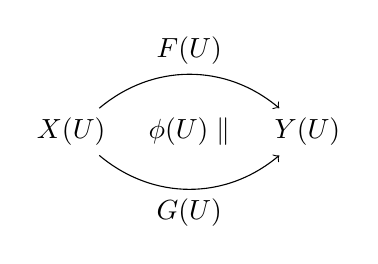
\begin{tikzpicture}
            % Nodes for X(U) and Y(U)
            \node (X) at (0,0) {$\mathfrak{X}(U)$};
            \node (Y) at (3,0) {$\mathfrak{Y}(U)$};

            % Top curved arrow
            \draw[->] (X) to[bend left=40] node[above] {$F(U)$} (Y);

            % Bottom curved arrow
            \draw[->] (X) to[bend right=40] node[below] {$G(U)$} (Y);

            % Middle label
            \node at (1.5,0) {$\phi(U)\parallel$};
        \end{tikzpicture}
    \]
    subject to some compatibility conditions.
\end{definition}

\begin{definition}[Fiber product, representable morphisms]
    Let $F: \mathfrak{X} \to \mathfrak{Y}$ be a morphism of $k$-stacks. The \textbf{fiber product} $\mathfrak{X}_\eta$ of $\mathfrak{X}$ over $\mathfrak{Y}$ at an object $\eta \in \mathfrak{Y}(U)$ is the $k$-stack defined by the rule
    \[
        \mathfrak{X}_\eta(V) = \mathfrak{X}(V) \times_{\mathfrak{Y}(V)} \{\eta|_V\}
    \]
    In particular, such an object $\eta$ can be thought of as a morphism $\eta: U \to \mathfrak{Y}$. Then the fiber of the morphism $F$ over $\eta$ is precisely the stack $\mathfrak{X} \times_{\mathfrak{Y}} U$.

    The morphism $F: \mathfrak{X} \to \mathfrak{Y}$ is \textbf{representable} if $\mathfrak{X}_\eta$ is representable as a scheme for all $U \in \ob(\mathbf{Aff}/k)$ and all $\eta \in \ob\mathfrak{Y}(U)$.



    We say $F$ has propety $P$ if for every $U \in \ob(\mathbf{Aff}/k)$ and every $\eta \in \ob(Y(\eta))$ the canonical morphism (coming from forming the fiber stack as a pullback) of schemes $\mathfrak{X}_\eta \to U$ has $P$.  Examples of such properties are flat, smooth, surjective, étale, etc.
\end{definition}

\begin{definition}
    A $k$-stack $\mathfrak{X}$ is \textbf{algebraic} if
    \begin{enumerate}
        \item[(i)] the diagonal morphism $\mathfrak{X} \to \mathfrak{X} \times \mathfrak{X}$ is representable, separated and quasi-compact
        \item[(ii)] there is a $k$-scheme $P$ and a smooth, surjective morphism $P \stackrel{p}{\to} \mathfrak{X}$.
    \end{enumerate}
\end{definition}

\begin{remark}
    Given any scheme $T$ with two maps $f, g : T \to \mathfrak{X}$ (representing two families of objects parameterized by $T$), the fiber product:
    \begin{align*}
        T \times_{(\mathfrak{X} \times \mathfrak{X})} \mathfrak{X} \cong \text{Isom}_T(f, g)
    \end{align*}
    represents the "scheme of isomorphisms" between the objects corresponding to $f$ and $g$.    The condition that $\Delta : \mathfrak{X} \to \mathfrak{X} \times \mathfrak{X}$ is representable means that for any scheme $T$ with a morphism $T \to \mathfrak{X} \times \mathfrak{X}$, the fiber product $T \times_{\mathfrak{X} \times \mathfrak{X}} \mathfrak{X}$ is (represented by) an algebraic space. This controls the "size" of automorphism groups.
\end{remark}

\subsection{Examples of algebraic stacks}
\begin{definition}
    Let $G$ be an algebraic group acting on a scheme $X$. The action groupoid $X/G$ is the category whose objects are the points of $X$ and morphisms from $x$ to $y$ are the elements of $G$ such that $gx = y$.
\end{definition} Note that the isomorphism classes of the action groupoid are in bijection with
the orbits of $G $ on $X$. There is a canonical map $X/G \to */G$ which is obvious on the level of groupoids.

\begin{definition}
    We define the quotient stack $X/G: \Sch \to \Gpd$ by \begin{align*}
        (X/G)(S) = \text{sheafification of the presheaf } S \mapsto X(S)/G(S)
    \end{align*}
\end{definition}
From the moduli perspective, we have to ask: what family over $S$ is parameterized by $(X/G)(S)$ for a test scheme $S$? We can answer this question as follows.

The first thing we notice is that the map $X \rightarrow *$ should induce a canonical map $X/G \rightarrow */G$. Thus an $S$-point of $S \rightarrow X/G$ induces by composition an $S$-point $S \rightarrow */G$; i.e., a $G$-torsor $P$ over $S$.

Now, say we have a $G$-torsor $P$ over $S$. We can form the fiber product:

\begin{center}
    \begin{tikzcd}
        X \times^G P \arrow[r] \arrow[d] & X/G \arrow[d] \\
        S \arrow[r, "P"] & */G
    \end{tikzcd}
\end{center}

We call the stack $X \times^G P$ the $X$-bundle associated to $P$, or the associated bundle of $P$ with
fiber $X$. In particular, there is the following correspondence:

\begin{proposition}
    There is a canonical bijection between:

    \begin{enumerate}
        \item Maps from a scheme $S$ to the quotient stack $X/G$
        \item Sections of the associated bundle $S \to X \times^G P$
        \item $G$-equivariant maps from $P$ to $X$
    \end{enumerate} where $P$ is the principal $G$-bundle on $S$ corresponding to $S \to X/G \to */G$.
\end{proposition}

\begin{proof}
    A map $f: S \to X/G$ of stacks corresponds to a principal $G$-bundle $P$ on $S$ together with a $G$-equivariant map $\phi: P \to X$. Given a $G$-equivariant map $\phi: P \to X$, we can construct a section $\sigma: S \to X \times^G P$ of the associated bundle as follows:

    For each point $s \in S$, define $\sigma(s) = [\phi(p), p]$ where $p$ is any point in the fiber $P_s$ and $[\phi(p), p]$ denotes the equivalence class in $X \times^G P$. The $G$-equivariance of $\phi$ ensures this is well-defined regardless of which $p \in P_s$ we choose.


    Conversely, given a section $\sigma: S \to X \times^G P$ where $\sigma(s) = [x_s, p_s]$ for each $s \in S$, we can define a $G$-equivariant map $\phi: P \to X$ as follows:

    For any $p \in P$ with $p \in P_s$ for some $s \in S$, we have $p = p_s \cdot g$ for some $g \in G$. We define $\phi(p) = g^{-1} \cdot x_s$. The properties of the associated bundle ensure this is well-defined and $G$-equivariant.
\end{proof}

This motivates the following definition:
\begin{definition}
    Let an algebraic group $G$ act on a scheme $X$. Then the \textbf{quotient stack} $X/G$ is the functor $\text{Sch} \to \text{Gpd}$ given by
    \begin{align*}
        (X/G)(S) = \text{Groupoid of principal $G$-torsors $P$ over $S$ with a $G$-equivariant map $P \to X$}.
    \end{align*}
\end{definition}


\begin{example}
    If $Z$ is a $k$-scheme and $H$ is a linear algebraic group over $k$ acting on $Z$, then the quotient stack $[Z/H]$ is an algebraic stack. A presentation is given by the trivial $H$-bundle $p:Z \to [Z/H]$.
\end{example}

\begin{example}
    Let $X$ be a projective connected smooth curve over $k$. The moduli problem $\mathcal{M}_{G,X}$ which associated to a scheme $S$ the groupoid of principal $G$-bundles over $X \times S$ is an algebraic stack. \begin{align*}
        \mathcal{M}_{G,X}(S):\Sch/k^{op} & \to \Gpd                                                                             \\
        S                                & \mapsto \{ \text{principal $G$-bundles over } X \times S \} + {\text{isomorphisms} }
    \end{align*}
\end{example}

\begin{proposition}
    If $G$ is reductive, the algebraic stack $\mathcal{M}_{G,X}$ is smooth, dimension $\dim G(g-1)$.
\end{proposition}

\section{Uniformization}
The theory of uniformization relates these moduli spaces to loop groups and associated Grassmannians. We introduce the uniformization of moduli stacks of principal $G$-bundles, beginning with the topological perspective and transitioning to the algebraic setting. 
\subsection{Topological loop groups}
Let $X$ be a smooth projective curve over $k$. Let $G$ connected reductive. Then isomorphism classes of topological principal $G$-bundles over $X$ are in bijection with elements of $\pi_1(G)$.

To see this, consider a basepoint $x\in X$ and a disk $D$ around $x$. Then the restriction of a principal $G$-bundle $P$ to $D$ is trivial because $D$ is contractible. Let $X^* = X \backslash \set{x}$. Then $U$ is homotopy equivalent to a wedge of circles and therefore any topological principal $G$-bundle over $U$ is also trivial. This is because of the general theory of obstruction theory for CW complexes.

In general, given a CW complex $X$ and a map from the $i$-skeleton $X^i \to Y$, the obstruction to extending this map to the $(i+1)$-skeleton lies in the cellular cohomology group $H^{i+1}(X^, \pi_i(Y))$. We also make use of the fact that a topological principal $G$-bundle $P$ over a space $X$ is trivial if and only if it admits a global section. In particular, to trivialize a principal $G$-bundle over $X$ is precisely to specify a map $X \to G$. Therefore, the obstruction to lifting a map $X^{*0} \to G$ to $X^{*1} \to G$ lies in the group $H^1(U, \pi_0(G))$ but $\pi_0(G) = e$ so this group is trivial. Therefore, all topological principal $G$-bundle over $U$ are trivial.

Another way to see this is using the theory of classifying spaces. Prinicipal $G$-bundles over $X^*$ are classified by homotopy classes of maps $X^* \to BG$. By the cellular approximation theorem, any map $X^* \to BG$ can be homotoped to a map $X^* \to BG^1$ where $BG^1$ is the 1-skeleton of $BG$. But $BG$ carries a cell structure with cells in only even dimensions, so such homotopy classes of maps amount to picking a connected component of $BG$. But $BG$ is connected because $G$ is connected. Therefore, all principal $G$-bundles over $U$ are trivial.

Return to $X$. The only data that is important, since the bundle is trivial over $X^*$ and $D$, is the transition function $g_{X^*D} \in G$. This amounts to a map $D^* = D \backslash \set{x} \to G$. But $D^*$ is homotopy equivalent to a circle, so this map is classified by an element of $\pi_1(G)$. Therefore, the isomorphism classes of principal $G$-bundles over $X$ are in bijection with $\pi_1(G)$.

We recast the argument given above:
\begin{definition}
    We have the following groups: \begin{align*}
        L^{top}G   & = \{ \text{continuous maps } D^* \to G \} \\
        L^{top}_+G & = \{ \text{continuous maps } D \to G \}   \\
        L^{top}_XG & = \{ \text{continuous maps } X^* \to G \}
    \end{align*} and natural inclusions $L^{top}_+G \to L^{top}G$ and $L^{top}_XG \to L^{top}G$.
\end{definition}
\begin{proposition}
    There is a canonical bijection \begin{align*}
        L^{top}_XG \backslash L^{top}G / L^{top}_+G \cong \mathcal{M}^{top}_{G,X} \cong \pi_1(G)
    \end{align*}
\end{proposition}

\begin{proof}
    One thinks of the space \begin{align*}
        L^{top}G = \{ E,\sigma,\tau \}
    \end{align*} of triples where $E \to X$ is a principal $G$ bundle and $\sigma:E\vert_D \cong D\times G$ and $\tau:E\vert_{X^*} \cong X^* \times G$ are choices of trivializations. Then one divides out by the choice of trivializations.
\end{proof}

\subsection{Algebraic loop groups}
The algebraic analagoue of a neighborhood homeomorphic to $x$ is given by looking at the completion of the local ring $\cO_{X,x}$. \begin{align*}
    D_x = \Spec \hat{\cO_{X,x}}
\end{align*} Choosing a local coordinate $z$ near $x$ gives the idenitfication \begin{align*}
    D_x = \Spec k[[z]]
\end{align*} The punctured disk is the field of fractions $K_x$ of the completion of the local ring \begin{align*}
    D_x^* = \Spec K_x \cong \Spec k((z))
\end{align*}
Introduce the notation $U = \Spec R$, $D_U^* = \Spec R((z))$ and $D_U = \Spec R[[z]]$ and $X^*_U = X^*\times U$.

The algebraic analogue of the topological loop group $L^{top}G$ is the group scheme \begin{align*}
    LG = \underline{\Hom}_{alg}(D^*, G)
\end{align*} the points of $G$ with values in $D^*$, i.e. $G(k((z)))$.
\begin{definition}
    We have the functor of points for \textbf{algebraic loop groups} \begin{align*}
        LG: \Aff/k & \to \Grp                           \\
        LG(U)      & = \Hom_{alg}(D_U^*, G) = G(R((z)))
    \end{align*} and the analagous $k$-groups \begin{align*}
        L_+G(U) & = \Hom_{alg}(D_U, G) = G(R[[z]])        \\
        L_XG(U) & = \Hom_{alg}(X^*_U, G) = G(\cO_{X^*_U})
    \end{align*} The quotient space $\cQ_G = LG/L_+G$ is the sheafification of the presheaf \begin{align*}
        U \mapsto LG(U)/L_+G(U)
    \end{align*} carries an action of $L_XG$.
\end{definition}
Consider the quotient stack $[L_XG\backslash \cQ_G]$.
\begin{theorem}[Uniformization]
    Let $G$ semisimple. Then there is a canonical isomorphism of stacks \begin{align*}
        [L_XG\backslash \cQ_G] \cong \mathcal{M}_{G,X}
    \end{align*} Moreover the $L_XG$-bundle $\cQ_G \to \cM_{G,X}$ is even locally trivial for the etale topology if the characteristic of $k$ does not divide the order of $\pi_1(G(\C))$.
\end{theorem}
We consider triples $(E, \rho, \sigma)$ where $E$ is a vector bundle on $X_R$, $\rho : \mathcal{O}^r_{X^*_R} \longrightarrow E|_{X^*_R}$ a trivialization of $E$ over $X^*_R$, $\sigma : \mathcal{O}^r_{D_R} \longrightarrow E|_{D_R}$ a trivialization of $E$ over $D_R$. We let $\textrm{T}(R)$ be the set of isomorphism classes of triples $(E, \rho, \sigma)$ (with the obvious notion of isomorphism).
\begin{proposition}
    The ind-group $\mathbf{GL}_r(K)$ represents the functor $\textrm{T}$.
\end{proposition}
\begin{proposition}
    The ind-group $\mathbf{SL}_r(K)$ represents the subfunctor $\textrm{T}_0$ of $\textrm{T}$ which associates to a $k$-algebra $\textrm{R}$ the set of isomorphism classes of triples $(E, \rho, \sigma)$ where $E$ is a vector bundle on $\textrm{X}_{\textrm{R}}$, $\rho : \mathcal{O}^r_{\textrm{X}^*_{\textrm{R}}} \longrightarrow E|_{\textrm{X}^*_{\textrm{R}}}$ and $\sigma : \mathcal{O}^r_{\textrm{D}_{\textrm{R}}} \longrightarrow E|_{\textrm{D}_{\textrm{R}}}$ are isomorphisms such that $\wedge^r \rho$ and $\wedge^r \sigma$ coincide over $\textrm{D}^*_{\textrm{R}}$.
\end{proposition}

\begin{remark}
    The condition that the trivializations $\wedge^r \rho$ and $\wedge^r \sigma$ coincide over $\textrm{D}^*_{\textrm{R}}$ means that they come from a global trivialization of $\wedge^r E$. So we can rephrase by saying that $\textrm{T}_0(R)$ is the set of isomorphism classes of data $(E, \rho, \sigma, \delta)$ where $\delta$ is a trivialization of $\wedge^r E$, $\rho$ and $\sigma$ are trivializations of $E|_{\textrm{X}^*_{\textrm{R}}}$ and $E|_{\textrm{D}_{\textrm{R}}}$, respectively, such that $\wedge^r \rho$ coincide with $\delta|_{\textrm{X}^*_{\textrm{R}}}$ and $\wedge^r \sigma$ with $\delta|_{\textrm{D}_{\textrm{R}}}$.
\end{remark}

\begin{corollary}
    Let us denote by $\textrm{A}_{\textrm{X}}$ the affine algebra $\Gamma(X - p, \cO_X)$. There is a canonical bijective correspondence between the set of isomorphism classes of rank $r$ vector bundles on $\textrm{X}$ with trivial determinant (resp. with determinant of the form $\cO_X(np)$ for some integer $n$) and the double coset space $\textrm{SL}_r(\textrm{A}_{\textrm{X}})\backslash \textrm{SL}_r(K)/\textrm{SL}_r(\mathcal{O})$ (resp. $\textrm{GL}_r(\textrm{A}_{\textrm{X}})\backslash \textrm{GL}_r(K)/\textrm{GL}_r(\mathcal{O})$).
\end{corollary}
\begin{proof}
    Since two trivializations of $E|_{\textrm{D}}$ differ by an element of $\textrm{GL}_r(\mathcal{O})$, and two trivializations of $E|_{\textrm{X}^*}$ by an element of $\textrm{GL}_r(\textrm{A}_{\textrm{X}})$,  bijection between $\textrm{GL}_r(\textrm{A}_{\textrm{X}})\backslash\textrm{GL}_r(K)/\textrm{GL}_r(\mathcal{O})$ and the set of isomorphism classes of rank $r$ vector bundles on $\textrm{X}$ which are trivial on $\textrm{X}^*$. But a projective module over a Dedekind ring is free if and only if its determinant is free, hence our assertion for $\textrm{GL}_r$. The same proof applies for $\textrm{SL}_r$.
\end{proof}
\begin{remark}
    Note that saying that a line bundle is trivial on the open complement $X^* = X - p$ is equivalent to saying that it is of the form $\mathcal{O}_{X}(np)$ for some integer $n$. This follows from the exact sequence \begin{align*}
        \Z \to \Pic(X) \to \Pic(X^*) \to 0
    \end{align*} where the first map sends $1 \mapsto \mathcal{O}_X(p)$.
\end{remark}

\begin{lemma}
    Let $G$ be any semisimple group. Given a principal $G$-bundle $\mathcal{E}$, and any representation $\rho : G \to \text{GL}(V)$, the contracted product $E = \mathcal{E} \times_G V$ has trivial determinant.
\end{lemma}

\begin{proof}
    To see that $\det(E)$ is trivial, we note that since $G$ is semisimple, $[G,G] = G$, and so the image $\rho(G)$ is contained in the kernel of the determinant map which is $\text{SL}(V)$. This is because $\rho$ preserves commutator subgroups and $[\GL_n, \GL_n] \subset \SL_n$.

    In particular, $E$ has transition functions given by matrices with trivial determinant. These are the transition functions of the line bundle $\det(E)$, and so $\det(E)$ is necessarily trivial.
\end{proof}

\subsection{As a moduli stack}
In the last section, we described a bijection between the set of isomorphism classes of rnak $r$ vector bundles on $X$ with trivial determinant and the double coset space $\SL_r(A_X) \backslash \SL_r(K) / \SL_r(\cO)$ by considering triples $(E,\sigma,\tau)$ corresponding to vector bundles $E$ along with choices of trivializations over the open complement of a point, and the unit disk respectively. This in fact gives a description of the moduli stack. This section is about understanding the algebraic structure of the stack $\SL_r(A_X) \backslash \SL_r(K) / \SL_r(\cO)$.

We begin with result about the infinite Grassmannian.
\begin{proposition}
    The $k$-space $\mathcal{Q} := \mathbf{SL}_r(K)/\mathbf{SL}_r(\mathcal{O})$ represents the functor which associates to a $k$-algebra $\textrm{R}$ the set of isomorphism classes of pairs $(E, \rho)$, where $E$ is a vector bundle over $\textrm{X}_{\textrm{R}}$ and $\rho$ a trivialization of $E$ over $\textrm{X}^*_{\textrm{R}}$ such that $\wedge^r \rho$ extends to a trivialization of $\wedge^r E$.
\end{proposition}

\begin{proof}
    A standard proof using descent. Let $R$ be a $k$-algebra and $q$ an element of $Q(R)$. By definition there exists a faithfully flat homomorphism $R \rightarrow R'$ and an element $\gamma$ of $\SL_r(R'((z)))$ such that the image of $q$ in $\cQ(R')$ is the class of $\gamma$. Effective, we are checking that the proposition holds for an fppf covering of $R$, and then it will necessarily hold for $R$ by descent.

    To $\gamma$ corresponds a triple $(E', \rho', \sigma')$ over $X_{R'}$. Let $R'' = R' \otimes_{R} R'$, and let $(E_1'', \rho_1''), (E_2'', \rho_2'')$ denote the pull-backs of $(E', \rho')$ by the two projections of $X_{R''}$ onto $X_{R'}$. Since the two images of $\gamma$ in $\SL_r(R''((z)))$ differ by an element of $\SL_r(R''[[z]])$, these pairs are isomorphic; this means that the isomorphism $\rho_2''\rho_1''^{-1}$ over $X_{R''}^*$ extends to an isomorphism $u: E_1'' \rightarrow E_2''$ over $X_{R''}$. This isomorphism satisfies the usual cocycle condition, because it is enough to check it over $X^*$, where it is obvious. Therefore $(E', \rho')$ descends to a pair $(E, \rho)$ on $X_{R}$ as in the statement of the proposition.

    Conversely, given a pair $(E, \rho)$ as above over $X_{R}$, we can find a faithfully flat homomorphism $R \rightarrow R'$ and a trivialization $\sigma'$ of the pull back of $E$ over $D_{R'}$ such that $\wedge^r\sigma'$ coincides with $\wedge^r\rho$ over $D_{R'}^*$ (in fact $\operatorname{Spec}(R)$ is covered by open subsets $\operatorname{Spec}(R_\alpha)$ such that $E$ is trivial over $D_{R_\alpha}$, and we can take $R' = \prod R_\alpha$). By prop. 1.5 we get an element $\gamma'$ of $\mathbf{SL}_r(R'((z)))$ such that the two images of $\gamma'$ in $\mathbf{SL}_r(R''((z)))$ (with $R'' = R' \otimes_{R} R'$) differ by an element of $\mathbf{SL}_r(R''[[z]])$; this gives an element of $Q(R)$. The two constructions are clearly inverse one of each other.
\end{proof}

\subsection{As a Grassmannian of lattices}
For any $k$-algebra $R$ define \textbf{lattice} in $R((z))^r$ as a sub-$R[[z]]$ module $W$ of $R((z))$ which is projective of rank $R$ and so that $\cup z^{-n}W = R((z))^r$. In particular this implies that \begin{align*}
    z^{-N}R[[z]] \subset W \subset z^N R[[z]]
\end{align*} for some integer $N$, and so that the $R$-module $W/z^NR[[z]]^r$ is projective. Moreover we say that the lattice $W$ is \textbf{special} if the projective $R$-module $W/z^NR[[z]]$ is of rank $Nr.$ This is equivalent to saying that the determinant $\Lambda^rW$ is trivial $= R[[z]]$.

\begin{proposition}
    The $k$-space $Q$ (resp. $\mathbf{GL}_r(\mathrm{K})/\mathbf{GL}_r(\mathcal{O})$) represents the functor which associates to a $k$-algebra $\mathrm{R}$ the set of special lattices (resp. of lattices) $\mathrm{W} \subset \mathrm{R}((z))^r$. The group $\mathbf{SL}_r(\mathrm{K})$ acts on $Q$ by $(\gamma, \mathrm{W}) \mapsto \gamma \mathrm{W}$ (for $\gamma \in \mathbf{GL}_r(\mathrm{R}((z)))$, $\mathrm{W} \subset \mathrm{R}((z))^r$).
\end{proposition}

\begin{center}
    \begin{tikzcd}
        \mathrm{D}^* \arrow[r, hook] \arrow[d] & \mathrm{D} \arrow[d] \\
        \mathrm{X}^* \arrow[r, hook] & \mathrm{X}
    \end{tikzcd}
\end{center}

\begin{proof}
    Consider the diagram where for simplicity we have dropped the suffix $R$. Let us start with a pair $(E, \rho)$ over $X$. The trivialization $\rho$ gives an isomorphism $R((z))^r \longrightarrow H^0(D^*, E|_{D^*})$; the inverse image $W$ of $H^0(D, E|_{D})$ is a lattice in $R((z))^r$, and it is a special lattice if $\wedge^r \rho$ extends to a trivialization of $\wedge^r E$ over $X$.

    Conversely, given a lattice $W$ in $R((z))^r$, we define a vector bundle $E_W$ on $X$ by gluing the trivial bundle over $X^*$ with the bundle on $D$ associated to the $R[[z]]$-module $W$; the gluing isomorphism is the map $W \otimes_{R[[z]]} R((z)) \longrightarrow R((z))^r$ induced by the embedding $W \hookrightarrow R((z))^r$. By definition $E_W$ has a natural trivialization $\rho_W$ over $X^*$, and if $W$ is a special lattice $\wedge^r \rho$ extends to a trivialization of $\wedge^r E$ over $X$. It is easy to check that these two constructions are inverse one of each other.

    Let $\gamma$ be an element of $\mathbf{GL}_r(R((z)))$, corresponding to a triple $(E, \rho, \sigma)$. By construction the corresponding lattice is $\rho^{-1} \sigma(R[[z]]^r) = \gamma(R[[z]]^r)$.
\end{proof}

Recall that we have denoted by $S^{(N)}$ the subscheme of $\mathrm{SL}_r(K)$ parametrizing matrices $A(z)$ such that $A(z)$ and $A(z)^{-1}$ have a pole of order $\leq N$; it is stable under right multiplication by $S^{(0)} = \mathrm{SL}_r(\mathcal{O})$. We will denote by $\mathcal{Q}^{(N)}$ its image in $\mathcal{Q}$, i.e. the quotient $k$-space $S^{(N)}/S^{(0)}$.

\vspace{10pt}

\begin{corollary}
    Let $\mathbb{F}_N$ be a free module of rank $r$ over the ring $k[z]/(z^{2N})$ (so that $\mathbb{F}_N$ is a $k$-vector space of dimension $2rN$). The $k$-space $\mathcal{Q}^{(N)} = S^{(N)}/S^{(0)}$ is isomorphic to the (projective) variety of $rN$-dimensional subspaces $G$ of $\mathbb{F}_N$ such that $zG \subset G$.
\end{corollary}
Recall that we have denoted by $\mathrm{SL}_r(\mathcal{O}_-)$ the subgroup of $\mathrm{SL}_r(k[z^{-1}])$ parametrizing matrices $\sum_{n \geq 0} A_n z^{-n}$ with $A_0 = \mathrm{I}$. It is an ind-variety.

\begin{theorem}
    The $k$-space $\mathcal{Q} = \mathrm{SL}_r(K)/\mathrm{SL}_r(\mathcal{O})$ is an ind-variety, direct limit of the system of projective varieties $(\mathcal{Q}^{(N)})_{N \geq 0}$. It is covered by open subsets which are isomorphic to $\mathrm{SL}_r(\mathcal{O}_-)$, and over which the fibration $p : \mathrm{SL}_r(K) \longrightarrow \mathcal{Q}$ is trivial.
\end{theorem}

\begin{proposition}
    Let $\omega$ be the class of the identity $I$ in $\cQ$.
    \begin{enumerate}
        \item The orbits of $\SL_r(\mathcal{O})$ in $\cQ$ are the orbits of the points $z^d\omega$ where $d$ runs through the sequences $d_1 \leq d_2 \leq \cdots \leq d_r$ and $\sum d_i = 0$.
        \item The orbit of $z^{d'}\omega$ is in the closure of $z^{d}\omega$ if and only if $d' \geq d$ in dominance order, i.e. the $p$th partial sum of $d'$ is greater than or equal to the $p$th partial sum of $d$ for all $p$.
    \end{enumerate}
\end{proposition}
\begin{proof}
    We have the formula \begin{align*}
        \begin{pmatrix}
            t^{-1}z & t^{-1} \\
            -t      & 0
        \end{pmatrix}\begin{pmatrix}
                         z^{d_1} & 0       \\
                         0       & z^{d_2}
                     \end{pmatrix}
        \begin{pmatrix}
            t & -t^{-1}z^{d_2 - d_1 - 1} \\
            0 & t^{-1}
        \end{pmatrix} = \begin{pmatrix}
                            z^{d_1+1}   & 0         \\
                            -t^2z^{d_2} & z^{d_2-1}
                        \end{pmatrix}
    \end{align*} and take the limit as $t \to 0$.
\end{proof}
\subsection{The moduli stack $\SL_r(A_X) \backslash \SL_r(K) / \SL_r(\mathcal{O})$}

Recall that a stack over $k$ associates to any $k$-algebra $R$ a groupoid $F(R)$, and to any morphism of $k$-algebras $u : R \to R'$ a functor $F(u) : F(R) \to F(R')$. This data should satisfy some compatibility conditions and as well as some localization properties.
\begin{example}
    The \textit{moduli stack} $\mathcal{G}\mathcal{L}_X(r)$ of rank $r$ vector bundles on X is defined by associating to a $k$-algebra $R$ the groupoid of rank $r$ vector bundles over $X_R$. Similarly, one defines a stack $\mathcal{S}\mathcal{L}_X(r)$ by associating to $R$ the groupoid of pairs $(E,\delta)$, where $E$ is a vector bundle over $X_R$ and $\delta : \mathcal{O}_{X_R} \to \bigwedge^r E$ an isomorphism; this is the fibre over the trivial bundle of the morphism of stacks $\det : \mathcal{G}\mathcal{L}_X(r) \to \mathcal{G}\mathcal{L}_X(1)$.
\end{example}

\begin{definition}
    A $\Gamma$-torsor over $R$ (in the fppf site) is a $k$-space $P$ over $R$ with an action of $\Gamma_R$ which after a faithfully flat extension $R\to R'$ becomes isomorphic to $\Gamma_{R'}$ acting on itself by multiplication.
\end{definition}

\begin{example}
    Let $Q$ be a $k$-space, and $\Gamma$ a $k$-group acting on $Q$. The quotient stack $\Gamma\backslash Q$ is defined in the following way: an object of $F(R)$ is a $\Gamma$-torsor $P$ over $\Spec R$ together with a $\Gamma$-equivariant morphism $\alpha : P \to Q$; arrows in $F(R)$ are defined in the obvious way, and so are the functors $F(u)$. The stack $\Gamma\backslash Q$ is indeed the quotient of $Q$ by $\Gamma$ in the category of stacks, in the sense that any $\Gamma$-invariant morphism from $Q$ into a stack $F$ factors through $\Gamma\backslash Q$ in a unique way. If $\Gamma$ acts freely on $Q$ (i.e. $\Gamma(R)$ acts freely on $Q(R)$ for each $k$-algebra $R$), then the stack $\Gamma\backslash Q$ is a $k$-space.
\end{example}

When $Q = \Spec(k)$ (with the trivial action), $\Gamma\backslash Q$ is the \textit{classifying stack} $B\Gamma$: for each $k$-algebra $R$, $B\Gamma(R)$ is the groupoid of $\Gamma$-torsors over $\Spec(R)$.

\begin{proposition}
    The quotient stack $\SL_r(A_X)\backslash\SL_r(K)/\SL_r(\mathcal{O})$ is canonically isomorphic to the algebraic stack $\mathcal{S}\mathcal{L}_X(r)$ of vector bundles on $X$ with trivial determinant. The projection map $\pi : \SL_r(K)/\SL_r(\mathcal{O}) \longrightarrow \mathcal{S}\mathcal{L}_r(X)$ is locally trivial for the Zariski topology.
\end{proposition}

\begin{example}
    [Determinant line bundle] Let $T$ be a scheme, and $E$ a vector bundle on $X \times T$. The derived direct image $R(pr_{T})_*(E)$ is given by a complex of vector bundles $L^0 \to L^1$.

    This is a complex which represents the higher direct image sheaves in the derived category, i.e. pass to a resolution of $E$ and take the pushforward. Since $X$ has dimension 1, we can represent this complex by a two term complex of vector bundles $L^0 \to L^1$.

    The line bundle $\det(L^1) \otimes \det(L^0)^{-1}$ is independent of the choice of this complex, hence canonically defined on $T$; this is the "determinant of the cohomology" $\det R\Gamma_{T}(E)$. The important thing to note here is that in the derived category, quasi-isomorphisms need not induce the same isomorphisms on cohomology. But they do induce the same isomorphism on determinants of cohomology. This is precisely the compatilibity we need to define the determinant line bundle for stacks, in particular we need to know that given quasi-isomorphic three complexes $K^*, L^*, M^*$, the composition of isomorphisms $\det K^* \to \det L^* \to \det M^*$ is the same as the isomorphism $\det K^* \to \det M^*$.

    Associating to each bundle $E$ on $X \times T$ the line bundle $\det R\Gamma_{T}(E)$ defines a line bundle $\mathcal{L}$ on the stack $\mathcal{S}\mathcal{L}_{X}(r)$ (or $\mathcal{G}\mathcal{L}_{X}(r)$), the \textit{determinant line bundle}.
\end{example}

\section{The central extension}
Recall that there is a canonical map of stacks $\pi:\cQ = \SL_r(K) / \SL_r(\mathcal{O}) \to \mathcal{SL}_X(r)$. Let $\cL$ be the determinant line bundle on $\mathcal{SL}_X(r)$. We are interested in relating the following central extension construction to the determinant bundle on the moduli stack.

\subsection{Fredholm group}
Let $V$ be an infinite dimensional vector space over $k$. Let $\End^f(V)$ denote the two sided ideal generated by the finite rank endomorphisms of $V$, and let $\cF(V) = (\End(V) / \End^f(V))^*$ be the equivalence classes of endomorphisms with finite dimensional kernel and cokernel. Let $\cF(V)^0$ denote the subgroup of index $0$ endomorphisms.

The map $\Aut(V) \hookrightarrow \End(V) \to \cF(V)$ has image precisely $\cF(V)^0$, and its kernel is those automorphisms $u \in \Aut(V)$ so that $u - I \in \End^f(V)$.
The determinant of such $u$ is well defined by the formula \begin{align*}
    \det(u) = \det(I+v) = \sum_{n\geq 0} \tr \Lambda^n v
\end{align*}
so there is a short exact sequence \begin{align*}
    0 \to I + \End^f(V) \to \Aut(V) \to \cF(V)^0 \to 0
\end{align*} Let $(I + \End^f(V))_1$ denote those automorphisms $u$ such that $\det(u) = 1$. We get a short exact sequence \begin{align*}
    0 \to k^* \to \Aut(V)/(I + \End^f(V))_1 \to \cF(V)^0 \to 0
\end{align*} For $v\in \End^f(V), u\in \Aut(V)$, we have \begin{align*}
    \det(I + uv\inv{u}) = \det(I + v)
\end{align*} so $\det(I+v)$ is invariant under conjugation and $I+v$ is in the center of $\Aut(V)/(I + \End^f(V))_1$. Thus we have defined a caonical central extension of the group $\cF(V)^0$ by $k^*$.

\subsection{Algebraic setting}
Consider the $k$-space $\End(V)(R) = \End_R(V\otimes_k R)$, and has the $k$-group $\Aut(V)$ as its group of units. An endomorphism of $V\otimes R$ has finite rank if its image is contained in a finitely generated submodule, denote these endomorphisms $\End^f(V)$ and take $\cF(V) = (\End(V) / \End^f(V))^*$. The group $\cF(V)^0$ is defined as the image of $\Aut(V)$ in $\cF(V)$. Then again there is a central extension \begin{align*}
    0 \to \Gm \to \Aut(V)/(I + \End^f(V))_1 \to \cF(V)^0 \to 0
\end{align*}

Now consider the ind-group $\GL_r(K)$. Choose a supplement $K^r = V \oplus \cO^r$ giving rise to a direct sum decomposition \begin{align*}
    R((z))^r = V \oplus R[[z]]^r
\end{align*} Let $\gamma \in \GL_r(R((z)))$ be a matrix with entries in $R((z))$ and decompose \begin{align*}
    \gamma = \begin{pmatrix}
                 a(\gamma) & b(\gamma) \\
                 c(\gamma) & d(\gamma)
             \end{pmatrix}
\end{align*}
so $a(\gamma):V_R \to V_R$ and consider the class $\bar{a}(\gamma) \in \End(V_R) / \End^f(V_R)$.

\begin{proposition}
    The map \begin{align*}
        \gamma \mapsto \bar{a}(\gamma)
    \end{align*} is a group homomorphism \begin{align*}
        \GL_r(R((z))) \to \cF(V_R)
    \end{align*} Another choice of supplement $V'$ gives rise to $\bar{a}':\GL_r(R((z))) \to \cF(V_R')$. Let $\phi:V \to V'$ be the map $V \to R((z))^r \to V'$. Then $\bar{a}'(\gamma) = \phi \circ \bar{a}(\gamma) \circ \phi^{-1}$.
\end{proposition}

\begin{proposition}
    Let $R$ be a $k$-algebra and $\gamma$ an element of $\text{SL}_r(R((z)))$; locally on $\text{Spec}(R)$ (for the Zariski topology), the endomorphism $a(\gamma)$ of $V_R$ is equivalent modulo $\End^f(V_R)$ to an automorphism.
\end{proposition}

It is enough to prove the result for one particular choice of $V$; we'll take $V = (z^{-1}k[z^{-1}])^r$. The assertion is clear when $\gamma$ belongs to $\text{SL}_r(R[[z]])$ or to $\text{SL}_r(R[z^{-1}])$: in those cases the matrix (4.2) is triangular, so that $a(\gamma)$ itself is an isomorphism. The result then follows when $R$ is a field, since any matrix $\gamma \in \text{SL}_r(R((z)))$ can be written as a product of elementary matrices $I + \lambda E_{ij}$, where $\lambda$ can be taken either in $R[[z]]$ or in $R[z^{-1}]$. The general case is a consequence of the following lemma:

\begin{lemma}
    Locally over $\text{Spec}(R)$, any element $\gamma$ of $\text{SL}_r(R((z)))$ can be written $\gamma_0\gamma^-\gamma^+$, with $\gamma_0 \in \text{SL}_r(K)$, $\gamma^- \in \text{SL}_r(R[z^{-1}])$, $\gamma^+ \in \text{SL}_r(R[[z]])$.
\end{lemma}

Let us assume first that the $k$-algebra $R$ is finitely generated. Let $t$ be a closed point of $\text{Spec}(R)$; put $\gamma_0 = \gamma(t)$. By (1.12) $\gamma_0^{-1}\gamma$ can be written in a neighborhood of $t$ as $\gamma^-\gamma^+$, hence the result in this case.

In the general case, $R$ is the union of its finitely generated subalgebras $R_\alpha$. Let \[p: \text{SL}_r(K) \longrightarrow \mathcal{Q} = \text{SL}_r(K)/\text{SL}_r(\mathcal{O})\] be the quotient map. Since $\mathcal{Q}$ is an ind-variety, the morphism $p \circ \gamma: \text{Spec}(R) \rightarrow \mathcal{Q}$ factors through $\text{Spec}(R_\alpha)$ for some $\alpha$. Locally over $\text{Spec}(R_\alpha)$, this morphism can be written $p \circ \gamma_\alpha$ for some element $\gamma_\alpha$ of $\text{SL}_r(R_\alpha((z)))$, which differs from $\gamma$ by an element of $\text{SL}_r(R[[z]])$ (thm.~2.5). Since $R_\alpha$ is of finite type, the lemma holds for $\gamma_\alpha$, hence also for $\gamma$.

\begin{corollary}
    The image of $\text{SL}_r(K)$ by $\bar{a}$ is contained in the subgroup $\mathcal{F}(V)^0$.
\end{corollary}

Take the pullback of the central extension \begin{align*}
    0 \to \Gm \to \Aut(V)/(I + \End^f(V))_1 \to \cF(V)^0 \to 0
\end{align*} by $\bar{a}$ so that we get \begin{align*}
    0 \to \Gm \to \hat\SL_r(K) \to \SL_r(K) \to 0
\end{align*} where $\hat\SL_r(K)$ is the central extension of $\SL_r(K)$ by $\Gm$. It is also an ind-group.

Explicitly, an element of $\SL_r(K)(R)$ is given, locally on $\Spec R$, by a pair $(\gamma, u)$ with $\gamma$ in $\SL_r(R((z)))$, $u$ in $\Aut(V_R)$, and $u \equiv a(\gamma)$ mod $\End^f(V_R)$. Two pairs $(\gamma, u)$ and $(\gamma', u')$ give the same element of $\hat\SL_r(K)(R)$ if $u^{-1}u'$ (which is in $I + \End^f(V_R)$) has determinant 1. The map \begin{align*}
    \psi: \hat\SL_r(K)(R) \longrightarrow \SL_r(K)(R)
\end{align*} is given by $\psi(\gamma, u) = \gamma$. The kernel of $\psi$ consists of the pairs $(I, u)$ with $u \in \Aut(V_R)$, modulo the pairs $(I, u)$ with $\det u = 1$; the map $u \mapsto \det u$ provides an isomorphism from $\ker \psi$ onto $\Gm(R)$.

\begin{remark}
    The interpretation of the central extension is as follows. Consider what happens when $\gamma \in \SL_r(R((z)))$ acts on $V_R$. The action $a(\gamma)$ is given by embedding $V_R$ into $R((z))^r$, and then applying the matrix $\gamma$ and projecting back to $V_R$. This map determined by $\gamma$ fails to be an automorphism, but we showed that if we perturb it by a finite rank endomorphism, we can get an automorphism. However we can get different automorphisms, and the central extension carries around the data of the particular automorphism we choose to represent the element $\gamma$. Two automorphisms are equivalent precisely when $\det(u^{-1}u') = 1$ which makes a $\Gm$-torsor.
\end{remark}

\begin{remark}
    Let $H$ be a sub-$k$-group of $\SL_r(K)$ such that $\mathcal{O}^r$ (resp. $V$) is stable under $H$. Then the extension $(\mathcal{E})$ is canonically split over $H$. For any element $\gamma \in H(R)$, we have $b(\gamma) = 0$ (resp. $c(\gamma) = 0$), so that the map $\gamma \mapsto a(\gamma)$ is a homomorphism from $H(R)$ into $\Aut(V_R)$. The map $\gamma \mapsto (\gamma, a(\gamma))$ defines a section of $\psi$ over $H$. In particular, the pullback $\widehat{\SL}_r(\mathcal{O})$ of $\SL_r(\mathcal{O})$ is canonically isomorphic to $\SL_r(\mathcal{O}) \times \Gm$.

    We denote by $\chi_0: \widehat{\SL}_r(\mathcal{O}) \to \Gm$ the second projection. If an element $\tilde{\delta} \in \widehat{\SL}_r(\mathcal{O})(R)$ is represented by a pair $(\delta, v)$, then
    \[
        \chi_0(\tilde{\delta}) = \det(a(\delta)^{-1} v).
    \]

    More generally, suppose there exists an element $\lambda \in \SL_r(K)$ such that the subgroup $H$ preserves the subspace $\lambda(\mathcal{O}^r)$ (resp. $\lambda(V)$). Choose an automorphism $u$ of $V$ such that $u \equiv a(\lambda) \pmod{\End^f(V)}$, and define a section of $\psi$ over $H$ by
    \[
        \gamma \mapsto (\gamma, ua(\lambda^{-1} \gamma \lambda)u^{-1}).
    \]
    This section is independent of the choice of $u$, so once again the group $H$ embeds canonically into $\widehat{\SL}_r(K)$.
\end{remark}

Let $\tilde{\gamma}$ an element of \( \widehat{\mathrm{SL}}_r(K)(R) \). Locally on \( \operatorname{Spec}(R) \) write \( \tilde{\gamma} = (\gamma, u) \) with \( \gamma \) in \( \mathrm{SL}_r(R((z))) \), \( u \in \mathrm{Aut}(V_R) \), and \( u \equiv a(\gamma) \pmod{\operatorname{End}^f(V_R)} \). We associate to this pair the element
\[
    \tau_V(\gamma, u) := \det(u a(\gamma^{-1}))
\]
of \( R \). This is clearly well-defined, so we get an algebraic function \( \tau_V \) on \( \widehat{\mathrm{SL}}_r(K) \).

\begin{proposition}
    Let $R$ be a $k$-algebra, $\tilde{\gamma}$ an element of $\widehat{\mathrm{SL}}_r(K)(R)$, $\gamma$ its image in $\mathrm{SL}_r(R((z)))$. One has
    \[
        \tau_V(\tilde{\gamma} \tilde{\delta}) = \chi_0(\tilde{\delta}) \tau_V(\tilde{\gamma})
    \]
    for all $\tilde{\delta}$ in $\widehat{\mathrm{SL}}_r(\mathcal{O})(R)$.
\end{proposition}


\begin{proof}
    Let us choose representatives \( (\gamma, u) \) of \( \tilde{\gamma} \) and \( (\delta, v) \) of \( \tilde{\delta} \). Since \( b(\delta^{-1}) = 0 \), one has
    \[
        a(\delta^{-1} \gamma \gamma^{-1}) = a(\delta^{-1}) a(\gamma^{-1}),
    \]
    and
    \[
        \tau_V(\tilde{\gamma} \tilde{\delta}) = \det (u v a(\delta^{-1}) a(\gamma^{-1})) = \det(v a(\delta^{-1})) \det(ua(\gamma^{-1})) = \chi_0(\tilde{\delta}) \tau_V(\tilde{\gamma}).
    \]
    as claimed.
\end{proof}

Let us denote by \( \chi \) the character \( \chi_0^{-1} \) of \( \widehat{\mathrm{SL}}_r(\mathcal{O}) \). The function \( \tau_V \) thus defines a section of the line bundle \( \mathcal{L}_{\chi} \) on the ind-variety
\[
    \cQ = \widehat{\mathrm{SL}}_r(K) / \widehat{\mathrm{SL}}_r(\mathcal{O})
\]
More generally, let \( \delta \in \mathrm{SL}_r(K) \), and let \( \tilde{\delta} \) be a lift of \( \delta \) in \( \widehat{\mathrm{SL}}_r(K) \); the function
\[
    \tilde{\gamma} \mapsto \tau_V(\tilde{\delta}^{-1} \tilde{\gamma})
\]
still defines an element of \( H^0(\cQ, \mathcal{L}_{\chi}) \), whose divisor is \( \delta(\operatorname{div}(\tau_V)) \).

\subsection{The determinant bundle}
We will now compare the pullback over $\cQ$ of the determinant line bundle $\cL$ on the moduli stack with the line bundle $\cL_\chi$.

\begin{proposition}
    Let $R$ be a $k$-algebra, $\gamma$ an element of $\GL_r(R((z)))$, and $(E,\rho,\sigma)$ the corresponding triple over $X_R$. There is a canonical exact sequence \begin{align*}
        0 \to H^0(X_R,E) \to A_X^r \otimes_k R \to (R((z))/R[[z]])^r \to H^1(X_R,E) \to 0
    \end{align*} where $\gamma: A_X^r \otimes_k R \to (R((z))/R[[z]])^r$ is the composition of the injection $A_X^r \otimes_k R \to R((z))^r$, the automorphism $\gamma^{-1}$ of $R((z))^r$, and the projection $R((z))^r \to (R((z))/R[[z]])^r$.
\end{proposition}
\begin{proof}
    Recall that there is a short exact sequence \begin{align*}
        0 \to \cO_X \to j_*O_{X^*} \to f_*(\cK_D/\cO_D) \to 0
    \end{align*} where $j: X^* \to X$ and $f: D \to X$ is the inclusion. The term $j_*O_{X^*}$ represents those sections of $O_X$ which are regular on $X^*$. The term $K_D/\cO_D$ represents the quotient of Laurent series by regular functions, and then we push it forward to $X$. The exact sequence says that a function on $X^*$ comes from a function on $X$ precisely when it has no poles along $D$. Tensoring with $E$ and using our trivializations $\rho,\sigma$ we get an exact sequence (tensoring with $E$ is exact because $E$ is locally free) \begin{align*}
        0 \to E \to j_*O_{X^*} \to f_*(\cK_D/\cO_D) \to 0
    \end{align*} Now take the long exact sequence in cohomology.
\end{proof}
Choose an element $\gamma_0\in \GL_r(K)$ so that $\bar{\gamma_0}:A_X^r \to (K/\cO)^r$ is an isomorphism, i.e. so that $E$ has no cohomology, i.e. so that $V = \gamma_0^{-1}(A_X^r)$ is a supplement of $\cO^r$ in $K^r$. Identifying $A_X^r$ with $V$ and the quotient map $K^r \to K^r/\cO^r$ with the projection of $K^r$ onto $V$, we obtain that $\bar{\gamma}$ is the composition of the mappings \begin{align*}
    V \to K^r \xrightarrow{\gamma^{-1}\gamma_0} K^r \to V
\end{align*} so that $\bar{\gamma}$ is the coefficient $a(\gamma^{-1}\gamma_0)$ of the matrix $\gamma^{-1}\gamma_0$ in the decomposition $K^r = V \oplus \cO^r$.

Therefore we have shown the following.
\begin{proposition}
    Let $\gamma \in \GL_r(R((z)))$, and let $E$ be the associated vector bundle over $X_R$. There is a canonical exact sequence:
    \begin{align*}
        0 \to H^0(X_R, E) \to V_R \xrightarrow{a(\gamma^{-1}\gamma_0)} V_R \to H^1(X_R, E) \to 0.
    \end{align*}
\end{proposition}

\begin{corollary}
    Assume that there exists an automorphism $u$ of $V_R$ such that $u \equiv a(\gamma_0^{-1}\gamma) \pmod{\End^f(V_R)}$. Then there is an exact sequence:
    \begin{align*}
        0 \to H^0(X_R, E) \to V_0 \xrightarrow{v_0} V_0 \to H^1(X_R, E) \to 0,
    \end{align*}
    where $V_0$ is a free finitely generated $R$-module, and $\det(v_0) = \tau_V(\gamma_0^{-1}\gamma, u)$.
\end{corollary}

\begin{proof}
    Let $v = u \cdot a(\gamma^{-1}\gamma_0) \in I + \End^f(V_R)$, and let $V_0$ be a free finitely generated direct factor of $V_R$ containing $\operatorname{Im}(v - I)$. Denote by $v_0$ the restriction of $v$ to $V_0$. The matrix of $v$ relative to a direct sum decomposition $V_R = V_0 \oplus V_1$ is of the form:
    \begin{align*}
        \begin{pmatrix}
            v_0 & * \\
            0   & I
        \end{pmatrix},
    \end{align*}
    from which it follows that $\det v_0 = \det v = \tau_V(\gamma_0^{-1}\gamma, u)$. It also follows that $\ker v_0 = \ker v$, and the inclusion $V_0 \hookrightarrow V_R$ induces an isomorphism $\operatorname{Coker} v_0 \cong \operatorname{Coker} v$.
\end{proof}

\begin{remark}
    One can think of the map $\tau_V(\gamma_0^{-1}\gamma,u)$ as a determinant associated with the difference between two ways of representing the action of $\gamma_0^{-1}\gamma$ on $V_R$. Specfically, when we have $u \equiv a(\gamma_0^{-1}\gamma) \pmod{\End^f(V_R)}$, the difference $u - a(\gamma_0^{-1}\gamma)$ is a finite rank endomorphism of $V_R$, and the determinant $\det(u - a(\gamma_0^{-1}\gamma))$ is well defined. The map $\tau_V$ is a way of encoding this information in a more algebraic form, and it allows us to compare different representations of the same action.

    The corollary says that we can "finitize" the cohomology computaiton to a finite-dimensional submodule $V_0$, and this localized computation preserves the key determinant information.
\end{remark}

\section{Appendix: Morphisms of Schemes}
Other notions for morphisms of schemes that we will not need, but still worth mentioning and defining.
\begin{definition}
    Let $f: X \to Y$ be a morphism of schemes.
    \begin{enumerate}
        \item $f$ is \textbf{affine} if for every affine open subset $V = \operatorname{Spec}(B) \subset Y$, the preimage $f^{-1}(V)$ is affine. Equivalently, there exists an affine open cover $\{V_i\}$ of $Y$ such that $f^{-1}(V_i)$ is affine for each $i$.
        \item $f: X \to Y$ is \textbf{finite} if for every affine open subset $V = \operatorname{Spec}(B) \subset Y$, the preimage $f^{-1}(V) = \operatorname{Spec}(A)$ where $A$ is a finite $B$-algebra (i.e., $A$ is finitely generated as a $B$-module).
        \item $f$ is \textbf{of finite type} if it is locally of finite type and quasi-compact.

        \item $f$ is \textbf{quasicompact} if for every quasi-compact open subset $V \subset Y$, the preimage $f^{-1}(V)$ is quasi-compact.
        \item $f: X \to Y$ is \textbf{separated} if the diagonal morphism $\Delta_f: X \to X \times_Y X$ is a closed immersion.
        \item $f: X \to Y$ is \textbf{quasi-separated} if the diagonal morphism $\Delta_f: X \to X \times_Y X$ is quasi-compact.
        \item $f: X \to Y$ is \textbf{proper} if it is separated, of finite type, and universally closed (the image of a closed subset remains closed after any base change).
        \item $f: X \to Y$ is \textbf{unramified} at a point $x \in X$ if:
              \begin{enumerate}
                  \item The extension of residue fields $\kappa(x)/\kappa(f(x))$ is finite and separable.
                  \item The cotangent space of the fiber at $x$, $\mathfrak{m}_{f(x)}\mathcal{O}_{X,x}/\mathfrak{m}_{f(x)}^2\mathcal{O}_{X,x}$, vanishes.
              \end{enumerate}
              It is \textbf{unramified} if it is unramified at every point of $X$.
        \item A morphism $f: X \to Y$ is \textbf{formally smooth} (resp. \textbf{formally unramified}, \textbf{formally étale}) if for every affine $Y$-scheme $Y' \to Y$ and every closed immersion $Y'_0 \to Y'$ defined by a nilpotent ideal, the map
              \begin{align*}
                  \operatorname{Hom}_Y(Y', X) \to \operatorname{Hom}_Y(Y'_0, X)
              \end{align*}
              is surjective (resp. injective, bijective).

        \item A morphism $f: X \to Y$ is \textbf{smooth} (resp. \textbf{unramified}, \textbf{étale}) if it is formally smooth (resp. formally unramified, formally étale) and locally of finite presentation.
        \item A morphism $f: X \to Y$ is \textbf{smooth} of relative dimension $n$ if it is flat, locally of finite presentation, and for each point $x \in X$, the fiber $X_{f(x)}$ is a smooth variety of dimension $n$ over $\kappa(f(x))$.
        \item A morphism $f: X \to Y$ is an \textbf{open immersion} if it induces a homeomorphism of $X$ onto an open subset of $Y$ and the induced map $f^\sharp: \mathcal{O}_Y|_{f(X)} \to f_*\mathcal{O}_X$ is an isomorphism.
        \item A morphism $f: X \to Y$ is a \textbf{closed immersion} if it induces a homeomorphism of $X$ onto a closed subset of $Y$ and the induced map $f^\sharp: \mathcal{O}_Y \to f_*\mathcal{O}_X$ is surjective.
        \item A morphism $f: X \to Y$ is \textbf{quasi-finite} at a point $x \in X$ if there exist open neighborhoods $U$ of $x$ and $V$ of $f(x)$ such that $f|_U: U \to V$ has finite fibers. It is \textbf{quasi-finite} if it is quasi-finite at every point of $X$.
    \end{enumerate}
\end{definition}

\begin{theorem}
    For a morphism of schemes $f: X \to Y$, the following are equivalent:
    \begin{enumerate}
        \item $f$ is formally smooth and locally of finite presentation.
        \item $f$ is flat, locally of finite presentation, and has geometrically regular fibers.
    \end{enumerate}
\end{theorem}

\begin{proof}
    We will prove both implications to establish the equivalence.

    \medskip
    \noindent \textbf{(1) $\Rightarrow$ (2):} Assume $f$ is formally smooth and locally of finite presentation.

    \medskip
    \noindent We need to establish that $f$ is flat and has geometrically regular fibers.

    \medskip
    \noindent \textbf{Step 1: Proving flatness.}

    \medskip
    \noindent Let $x \in X$ be a point and $y = f(x) \in Y$. We need to show that $\mathcal{O}_{X,x}$ is flat as an $\mathcal{O}_{Y,y}$-module. By standard criteria for flatness, it suffices to show that for every finitely generated ideal $I \subset \mathcal{O}_{Y,y}$, the natural map
    \begin{equation}
        \varphi: I \otimes_{\mathcal{O}_{Y,y}} \mathcal{O}_{X,x} \to I\mathcal{O}_{X,x}
    \end{equation}
    is an isomorphism, or equivalently, that $\text{Tor}_1^{\mathcal{O}_{Y,y}}(\mathcal{O}_{Y,y}/I, \mathcal{O}_{X,x}) = 0$.

    \medskip
    \noindent Since $f$ is formally smooth, by definition, for every affine $Y$-scheme $Y'$, every closed subscheme $Y'_0 \subset Y'$ defined by a nilpotent ideal $J$, and every $Y$-morphism $g_0: Y'_0 \to X$, there exists a $Y$-morphism $g: Y' \to X$ extending $g_0$.

    \medskip
    \noindent For our purposes, we consider the specific case where:
    \begin{align}
        Y'   & = \text{Spec}(\mathcal{O}_{Y,y}/I^2) \\
        Y'_0 & = \text{Spec}(\mathcal{O}_{Y,y}/I)
    \end{align}

    \noindent The ideal $J = I/I^2$ is nilpotent in $\mathcal{O}_{Y,y}/I^2$ with $J^2 = 0$.

    \medskip
    \noindent The obstruction to lifting $g_0: Y'_0 \to X$ to $g: Y' \to X$ lies in
    \begin{equation}
        \text{Ext}^1_{\mathcal{O}_{Y'_0}}(g_0^*L_{X/Y}, I/I^2)
    \end{equation}
    where $L_{X/Y}$ is the cotangent complex of $f$.

    \medskip
    \noindent Since $f$ is formally smooth, this obstruction vanishes for all possible $g_0$. Moreover, as $f$ is locally of finite presentation, the cotangent complex $L_{X/Y}$ is perfect and concentrated in degrees $[-1,0]$.

    \medskip
    \noindent By deformation theory, there is a connection between these Ext groups and the Tor groups relevant to flatness. Specifically, the vanishing of the obstruction for all $g_0$ implies that
    \begin{equation}
        \text{Tor}_1^{\mathcal{O}_{Y,y}}(\mathcal{O}_{Y,y}/I, \mathcal{O}_{X,x}) = 0
    \end{equation}

    This connection is established through the local-to-global spectral sequence relating Ext groups of the cotangent complex to appropriate Tor groups. For a formally smooth morphism, the cotangent complex is quasi-isomorphic to the module of differentials placed in degree 0, which simplifies these relationships.

    \medskip
    \noindent As this holds for all finitely generated ideals $I \subset \mathcal{O}_{Y,y}$, we conclude that $\mathcal{O}_{X,x}$ is flat over $\mathcal{O}_{Y,y}$. Since this applies to all points $x \in X$, the morphism $f$ is flat.


    \red{I am not confident in the truth of what is written here. It is also not complete.}
\end{proof}


\begin{remark}[Properties of morphisms]
    The following properties of morphisms of schemes are related in the following way:
    \begin{enumerate}
        \item finite $\Rightarrow$ proper $\Rightarrow$ separated
        \item finite $\Rightarrow$ affine $\Rightarrow$ quasi-affine
        \item finite $\Rightarrow$ quasi-finite
        \item étale $\Rightarrow$ smooth $\Rightarrow$ flat
        \item étale $\Rightarrow$ unramified
        \item locally of finite presentation $\Rightarrow$ locally of finite type
        \item proper + flat + finite type + locally of finite presentation $\Rightarrow$ cohomologically flat
    \end{enumerate}

    Properties preserved under composition include: affine, finite, (locally) of finite type, (locally) of finite presentation, quasi-compact, separated, proper, closed immersion, and flat.

    Properties preserved under base change include: affine, finite, (locally) of finite type, (locally) of finite presentation, flat, unramified, étale, smooth, open immersion, closed immersion, and proper.
\end{remark}

\section{Appendix: Associated Bundles}

Let $G$ be a group scheme and let $P \to X$ be a principal $G$-bundle over a scheme $X$. Suppose we have a scheme $F$ equipped with a (left) $G$-action. We can construct the associated bundle with fiber $F$, denoted $P \times^G F$, as follows.

Consider the product $P \times F$ with the diagonal $G$-action given by $g \cdot (p, f) = (p \cdot g^{-1}, g \cdot f)$ for $g \in G$, $p \in P$, and $f \in F$. The associated bundle $P \times^G F$ is defined as the quotient of $P \times F$ by this $G$-action:
\begin{align*}
    P \times^G F = (P \times F)/G
\end{align*}
More precisely, $P \times^G F$ can be constructed as the sheafification of the presheaf quotient $(P \times F)/G$ in the appropriate topology (étale, fppf, etc.). This construction yields a bundle $\pi: P \times^G F \to X$ where the fiber over each point $x \in X$ is isomorphic to $F$.

We can also go in the other direction - starting from a bundle with fiber $F$ and constructing a principal bundle.

\begin{definition}[Frame Bundle]
    Let $\pi: E \to X$ be a bundle whose fibers are isomorphic to a scheme $F$ on which $G$ acts. The \textbf{frame bundle} of $E$, denoted $\text{Fr}_G(E)$, is the $X$-scheme representing the functor that assigns to each $X$-scheme $T$ the set of $G$-equivariant isomorphisms:
    \begin{align*}
        \text{Fr}_G(E)(T) = \{\phi: T \times F \stackrel{\sim}{\to} E \times_X T \text{ (as $T$-schemes) } | \text{ $\phi$ is $G$-equivariant}\}
    \end{align*}
\end{definition}

\begin{proposition}
    Let $\pi: E \to X$ be a bundle with fiber $F$.
    \begin{enumerate}
        \item The frame bundle $\text{Fr}_G(E)$ is a principal $G$-bundle over $X$.
        \item If $E = P \times^G F$ is an associated bundle for some principal $G$-bundle $P$, then $\text{Fr}_G(E) \cong P$.
        \item For any bundle $E$ with fiber $F$, we have $E \cong \text{Fr}_G(E) \times^G F$.
    \end{enumerate}
\end{proposition}

This establishes a correspondence between principal $G$-bundles and bundles with fiber $F$ (with $G$-action), showing that these two perspectives are equivalent.

\begin{example}
    Let $E \to X$ be a vector bundle of rank $n$. Then the frame bundle $\text{Fr}_{\text{GL}_n}(E)$ is the principal $\text{GL}_n$-bundle whose fiber at $x \in X$ consists of all bases of the vector space $E_x$. Conversely, given a principal $\text{GL}_n$-bundle $P$, the associated bundle $P \times^{\text{GL}_n} \mathbb{A}^n$ is a vector bundle of rank $n$.
\end{example}


\section{References}
\begin{enumerate}
    \bibitem{BeauvilleLaszlo1994}
    Beauville, A., and Laszlo, Y.,
    \textit{Conformal blocks and generalized theta functions},
    \textit{Communications in Mathematical Physics},
    vol. 164, no. 2, pp. 385--419, 1994.

    \bibitem{Olsson2016}
    Olsson, M. C.,
    \textit{Algebraic Spaces and Stacks},
    American Mathematical Society Colloquium Publications, vol. 62,
    American Mathematical Society, Providence, RI, 2016.

    \bibitem{Sorger1999}
    Sorger, C.,
    \textit{Lectures on moduli of principal $G$-bundles over algebraic curves},
    in \textit{School on Algebraic Geometry (Trieste, 1999)}, pp. 1--57,
    ICTP Lecture Notes, vol. 1, Abdus Salam International Centre for Theoretical Physics, Trieste, 1999.
\end{enumerate}

\end{document}